% EIE330 Lab 1: editable group report.
% Self-contained: all diagrams and waveform data are embedded below.
% Saved experiment evidence is unchanged; this conversion does not rerun RTL.
% Names, IDs and completed full-workflow participation confirmed by the group.
\documentclass[10pt,a4paper]{article}
\usepackage[margin=20mm,top=18mm,bottom=22mm]{geometry}
\usepackage[T1]{fontenc}
\usepackage{lmodern}
\usepackage{amsmath,array,booktabs,xcolor,graphicx,tikz,fancyhdr}
\usepackage[hidelinks]{hyperref}
\urlstyle{same}
\setlength{\emergencystretch}{2em}
\setlength{\parindent}{0pt}
\setlength{\parskip}{5pt}
\renewcommand{\baselinestretch}{1.12}
\setlength{\headheight}{14pt}
\pagestyle{fancy}
\fancyhf{}
\renewcommand{\headrulewidth}{0pt}
\fancyfoot[L]{\footnotesize EIE330 | Group 10 | Lab 1}
\fancyfoot[R]{\footnotesize\thepage}
\hypersetup{pdftitle={EIE330 Lab 1 - Group Report},pdfauthor={Yu Zhihan, Jiang Yaxi, Zhang Hankun}}
\begin{document}


\vspace*{65.1968503937008pt}

\section*{EIE330 FPGA-based System Design}

{\LARGE\bfseries Lab 1-1: Full Adder\par}\vspace{5mm}

Group 10 - three-member group\par

\vspace*{19.84251968503937pt}

\begingroup\small\setlength{\tabcolsep}{4pt}
\renewcommand{\arraystretch}{1.20}
\noindent\begin{tabular}{@{}p{\dimexpr0.117647\linewidth-1.8824pt\relax}p{\dimexpr0.529412\linewidth-8.4706pt\relax}p{\dimexpr0.352941\linewidth-5.6471pt\relax}@{}}
\toprule
\textbf{Member} & \textbf{Name} & \textbf{Student ID} \\
\midrule
1 & Yu Zhihan & 1240029016 \\
2 & Jiang Yaxi & 1240006481 \\
3 & Zhang Hankun & 1240006465 \\
\bottomrule
\end{tabular}\par\endgroup
\vspace{2mm}

{\small\raggedright Cover information for Lab 1-1.\par}

\subsection*{Experiment scope}

This report presents the full-adder and one-bit comparator experiments, including circuit design, implementation, functional simulation, virtual-board verification and results.\par

The recorded tests use software simulation and a virtual board. Physical FPGA confirmation has not been completed.\par

\clearpage

\section*{Lab 1-1 | Introduction and requirements}

A full adder adds A, B and a carry-in Cin. Its outputs are the sum S and carry-out Cout. Unlike a half adder, it includes a carry from the previous bit, so it can be used in multi-bit addition [8].\par

The aim is to implement this function using board buttons and LEDs. The design is one combinational module with active-low input and output pins. All 8 required truth-table cases matched the simulated expectations and all 8 visible virtual-board cases passed. Table 1-1.1 summarizes the hardware constraints.\par

\subsection*{Member contributions}

All three members participated in the complete workflow for both the full-adder and one-bit comparator experiments. Their shared work included requirements and datasheet review; circuit specifications, active-low interfaces and port mapping; truth tables, Boolean equations, block diagrams and expected-waveform review; RTL and testbench preparation; compilation, synthesis and RTL inspection; functional simulation, waveform comparison and simulation-time analysis; the required virtual-board cases and recordings; and report preparation, references, links and group review.\par

- Yu Zhihan (1240029016): participated in every stage of both experiments, from requirements and circuit design through implementation, testing and report preparation. Cross-checked the Boolean equations, RTL and active-low port mapping.\\
- Jiang Yaxi (1240006481): participated in every stage of both experiments, from requirements and circuit design through implementation, testing and report preparation. Cross-checked the testbench stimuli, expected outputs and simulation waveforms.\\
- Zhang Hankun (1240006465): participated in every stage of both experiments, from requirements and circuit design through implementation, testing and report preparation. Cross-checked the virtual-board observations, recordings, report figures, references and links.\par

\subsection*{AI use}

AI assistance was used for RTL/testbench drafting, verification and simulator input support, and report text/figures. All three members reviewed the AI-assisted material.\par

\subsection*{Group cross-check}

The three members cross-checked both circuits and compared the expected outputs with the simulation and virtual-board results. They checked all eight full-adder combinations and all four comparator combinations, then reviewed the consistency of the equations, RTL, interface polarity, waveforms, LED observations and report.\par

\subsection*{Design constraints}

\begingroup\small\setlength{\tabcolsep}{4pt}
\renewcommand{\arraystretch}{1.20}
\noindent\begin{tabular}{@{}p{\dimexpr0.176471\linewidth-1.4118pt\relax}p{\dimexpr0.823529\linewidth-6.5882pt\relax}@{}}
\toprule
\textbf{Item} & \textbf{Constraint} \\
\midrule
FPGA & Cyclone IV E EP4CE10F17C8N [2], [4] \\
Capacity & 10,320 logic elements; 179 user I/O pins in a 256-pin package [3] \\
Buttons & Released pin = 1, pressed pin = 0; nominal 3.3 V pull-up [2], [4] \\
LEDs & Pin 0 turns an LED on; pin 1 turns it off [1], [2] \\
Clock & Board clock is 50 MHz; this combinational circuit needs no clock or stored state [2] \\
\bottomrule
\end{tabular}\par\endgroup
\vspace{2mm}

{\small\raggedright Table 1-1.1. Hardware constraints used for the design.\par}

\clearpage

\section*{Lab 1-1 | Specification and system design}

Logical input 1 means pressed; logical output 1 means illuminated. Ports ending in \_n use the opposite pin value. Table 1-1.2 gives every port and its board-model connection [2]; Table 1-1.3 defines the complete function.\par

\begingroup\small\setlength{\tabcolsep}{4pt}
\renewcommand{\arraystretch}{1.20}
\noindent\begin{tabular}{@{}p{\dimexpr0.247059\linewidth-5.9294pt\relax}p{\dimexpr0.129412\linewidth-3.1059pt\relax}p{\dimexpr0.288235\linewidth-6.9176pt\relax}p{\dimexpr0.335294\linewidth-8.0471pt\relax}@{}}
\toprule
\textbf{Port (1 bit)} & \textbf{Direction} & \textbf{Active level} & \textbf{Board signal / label} \\
\midrule
btn\_a\_n & Input & 0 = A pressed & B2 / KEY1 \\
btn\_b\_n & Input & 0 = B pressed & B3 / KEY2 \\
btn\_cin\_n & Input & 0 = Cin pressed & B4 / KEY3 \\
led\_s\_n & Output & 0 = S LED on & led1 / LED0 \\
led\_cout\_n & Output & 0 = Cout LED on & led2 / LED1 \\
\bottomrule
\end{tabular}\par\endgroup
\vspace{2mm}

{\small\raggedright Table 1-1.2. Ports of full\_adder\_lab and board-model mapping.\par}

\begingroup\small\setlength{\tabcolsep}{4pt}
\renewcommand{\arraystretch}{1.20}
\noindent\begin{tabular}{@{}p{\dimexpr0.441176\linewidth-3.5294pt\relax}p{\dimexpr0.558824\linewidth-4.4706pt\relax}@{}}
\toprule
\textbf{Logical inputs} & \textbf{Expected S, Cout} \\
\midrule
0 0 0 & 0 0 \\
0 0 1 & 1 0 \\
0 1 0 & 1 0 \\
0 1 1 & 0 1 \\
1 0 0 & 1 0 \\
1 0 1 & 0 1 \\
1 1 0 & 0 1 \\
1 1 1 & 1 1 \\
\bottomrule
\end{tabular}\par\endgroup
\vspace{2mm}

{\small\raggedright Table 1-1.3. Complete required truth table; output 1 means LED on.\par}

Figure 1-1.1 labels the structure and all signals. No other board input connects to the task module.\par

\begin{center}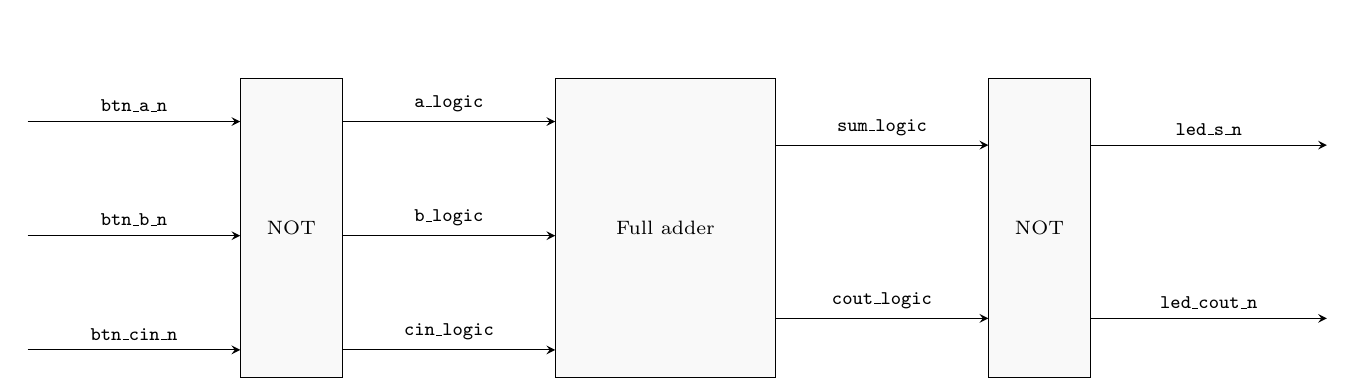
\begin{tikzpicture}[x=1cm,y=1cm,>=stealth,font=\scriptsize]
\path[use as bounding box] (0,0) rectangle (16.5,4.2);
\draw[fill=gray!5] (2.7,.25) rectangle (4.0,4.05);
\node at (3.35,2.15) {NOT};
\draw[fill=gray!5] (6.7,.25) rectangle (9.5,4.05);
\node at (8.1,2.15) {Full adder};
\draw[fill=gray!5] (12.2,.25) rectangle (13.5,4.05);
\node at (12.85,2.15) {NOT};
\draw[->] (0,3.5) -- (2.7,3.5);
\node[above] at (1.35,3.5) {\texttt{btn\_a\_n}};
\draw[->] (4,3.5) -- (6.7,3.5);
\node[above] at (5.35,3.5) {\texttt{a\_logic}};
\draw[->] (0,2.05) -- (2.7,2.05);
\node[above] at (1.35,2.05) {\texttt{btn\_b\_n}};
\draw[->] (4,2.05) -- (6.7,2.05);
\node[above] at (5.35,2.05) {\texttt{b\_logic}};
\draw[->] (0,0.6) -- (2.7,0.6);
\node[above] at (1.35,0.6) {\texttt{btn\_cin\_n}};
\draw[->] (4,0.6) -- (6.7,0.6);
\node[above] at (5.35,0.6) {\texttt{cin\_logic}};
\draw[->] (9.5,3.2) -- (12.2,3.2);
\node[above] at (10.85,3.2) {\texttt{sum\_logic}};
\draw[->] (13.5,3.2) -- (16.5,3.2);
\node[above] at (15.0,3.2) {\texttt{led\_s\_n}};
\draw[->] (9.5,1) -- (12.2,1);
\node[above] at (10.85,1) {\texttt{cout\_logic}};
\draw[->] (13.5,1) -- (16.5,1);
\node[above] at (15.0,1) {\texttt{led\_cout\_n}};
\end{tikzpicture}\end{center}

{\small\raggedright Figure 1-1.1. Input inversion, combinational logic and output inversion.\par}

The equations are S = A XOR B XOR Cin and Cout = (A AND B) OR (A AND Cin) OR (B AND Cin).\par

Continuous dataflow assignments are suitable because the outputs depend only on the current inputs. One module is sufficient for this small circuit. Input and output inversion satisfy the active-low board interface.\par

Traceability: the port table defines input/output polarity; the truth table defines the function; the block diagram implements it. The simulation rows and board checklist test the same cases.\par

\clearpage

\section*{Lab 1-1 | Implementation}

Figure 1-1.2 gives the expected initial sequence, holding each case for 10 ns. It is a report reference reconstructed from the truth table, not a preserved pre-coding student drawing.\par

\begin{center}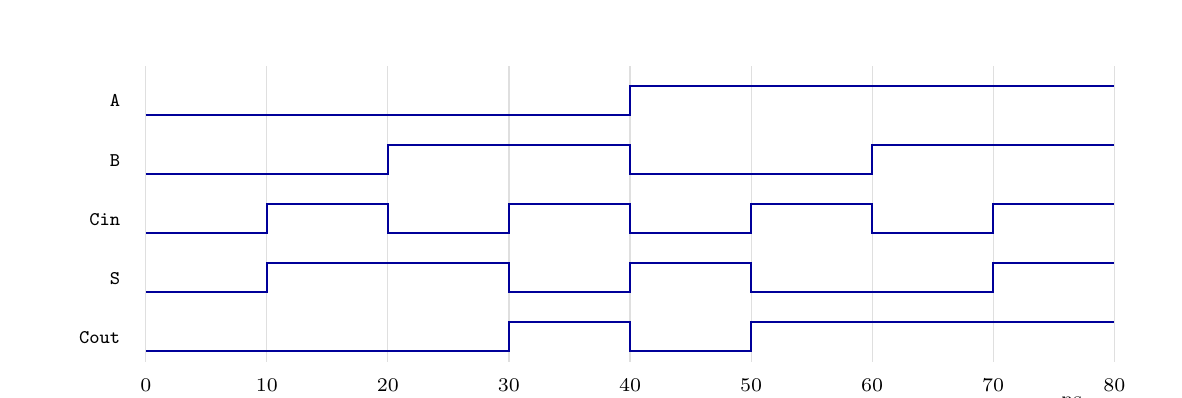
\begin{tikzpicture}[x=1cm,y=1cm,font=\scriptsize]
\path[use as bounding box] (-1.5,-.6) rectangle (12.8,3.75);
\draw[gray!25] (0.0,0) -- (0.0,3.75);
\node[below] at (0.0,-.1) {0};
\draw[gray!25] (1.5375,0) -- (1.5375,3.75);
\node[below] at (1.5375,-.1) {10};
\draw[gray!25] (3.075,0) -- (3.075,3.75);
\node[below] at (3.075,-.1) {20};
\draw[gray!25] (4.612500000000001,0) -- (4.612500000000001,3.75);
\node[below] at (4.612500000000001,-.1) {30};
\draw[gray!25] (6.15,0) -- (6.15,3.75);
\node[below] at (6.15,-.1) {40};
\draw[gray!25] (7.6875,0) -- (7.6875,3.75);
\node[below] at (7.6875,-.1) {50};
\draw[gray!25] (9.225000000000001,0) -- (9.225000000000001,3.75);
\node[below] at (9.225000000000001,-.1) {60};
\draw[gray!25] (10.762500000000001,0) -- (10.762500000000001,3.75);
\node[below] at (10.762500000000001,-.1) {70};
\draw[gray!25] (12.3,0) -- (12.3,3.75);
\node[below] at (12.3,-.1) {80};
\node[anchor=east] at (-.2,3.31) {\texttt{A}};
\draw[blue!60!black,line width=.7pt] (0.0000,3.1300) -- (0.0000,3.1300) -- (0.0000,3.1300) -- (1.5375,3.1300) -- (1.5375,3.1300) -- (1.5375,3.1300) -- (3.0750,3.1300) -- (3.0750,3.1300) -- (3.0750,3.1300) -- (4.6125,3.1300) -- (4.6125,3.1300) -- (4.6125,3.1300) -- (6.1500,3.1300) -- (6.1500,3.1300) -- (6.1500,3.5000) -- (7.6875,3.5000) -- (7.6875,3.5000) -- (7.6875,3.5000) -- (9.2250,3.5000) -- (9.2250,3.5000) -- (9.2250,3.5000) -- (10.7625,3.5000) -- (10.7625,3.5000) -- (10.7625,3.5000) -- (12.3000,3.5000);
\node[anchor=east] at (-.2,2.56) {\texttt{B}};
\draw[blue!60!black,line width=.7pt] (0.0000,2.3800) -- (0.0000,2.3800) -- (0.0000,2.3800) -- (1.5375,2.3800) -- (1.5375,2.3800) -- (1.5375,2.3800) -- (3.0750,2.3800) -- (3.0750,2.3800) -- (3.0750,2.7500) -- (4.6125,2.7500) -- (4.6125,2.7500) -- (4.6125,2.7500) -- (6.1500,2.7500) -- (6.1500,2.7500) -- (6.1500,2.3800) -- (7.6875,2.3800) -- (7.6875,2.3800) -- (7.6875,2.3800) -- (9.2250,2.3800) -- (9.2250,2.3800) -- (9.2250,2.7500) -- (10.7625,2.7500) -- (10.7625,2.7500) -- (10.7625,2.7500) -- (12.3000,2.7500);
\node[anchor=east] at (-.2,1.8099999999999998) {\texttt{Cin}};
\draw[blue!60!black,line width=.7pt] (0.0000,1.6300) -- (0.0000,1.6300) -- (0.0000,1.6300) -- (1.5375,1.6300) -- (1.5375,1.6300) -- (1.5375,2.0000) -- (3.0750,2.0000) -- (3.0750,2.0000) -- (3.0750,1.6300) -- (4.6125,1.6300) -- (4.6125,1.6300) -- (4.6125,2.0000) -- (6.1500,2.0000) -- (6.1500,2.0000) -- (6.1500,1.6300) -- (7.6875,1.6300) -- (7.6875,1.6300) -- (7.6875,2.0000) -- (9.2250,2.0000) -- (9.2250,2.0000) -- (9.2250,1.6300) -- (10.7625,1.6300) -- (10.7625,1.6300) -- (10.7625,2.0000) -- (12.3000,2.0000);
\node[anchor=east] at (-.2,1.06) {\texttt{S}};
\draw[blue!60!black,line width=.7pt] (0.0000,0.8800) -- (0.0000,0.8800) -- (0.0000,0.8800) -- (1.5375,0.8800) -- (1.5375,0.8800) -- (1.5375,1.2500) -- (3.0750,1.2500) -- (3.0750,1.2500) -- (3.0750,1.2500) -- (4.6125,1.2500) -- (4.6125,1.2500) -- (4.6125,0.8800) -- (6.1500,0.8800) -- (6.1500,0.8800) -- (6.1500,1.2500) -- (7.6875,1.2500) -- (7.6875,1.2500) -- (7.6875,0.8800) -- (9.2250,0.8800) -- (9.2250,0.8800) -- (9.2250,0.8800) -- (10.7625,0.8800) -- (10.7625,0.8800) -- (10.7625,1.2500) -- (12.3000,1.2500);
\node[anchor=east] at (-.2,0.31) {\texttt{Cout}};
\draw[blue!60!black,line width=.7pt] (0.0000,0.1300) -- (0.0000,0.1300) -- (0.0000,0.1300) -- (1.5375,0.1300) -- (1.5375,0.1300) -- (1.5375,0.1300) -- (3.0750,0.1300) -- (3.0750,0.1300) -- (3.0750,0.1300) -- (4.6125,0.1300) -- (4.6125,0.1300) -- (4.6125,0.5000) -- (6.1500,0.5000) -- (6.1500,0.5000) -- (6.1500,0.1300) -- (7.6875,0.1300) -- (7.6875,0.1300) -- (7.6875,0.5000) -- (9.2250,0.5000) -- (9.2250,0.5000) -- (9.2250,0.5000) -- (10.7625,0.5000) -- (10.7625,0.5000) -- (10.7625,0.5000) -- (12.3000,0.5000);
\node[anchor=west] at (11.5,-.5) {ns};
\end{tikzpicture}\end{center}

{\small\raggedright Figure 1-1.2. Expected logical input/output waveforms.\par}

The design is stored in RTL/ and the testbench in sim/ in the project bundle. A short implementation excerpt is shown below. The course requires publishing the complete RTL and testbench through GitHub [1].\par

\begin{verbatim}
assign sum_logic = a_logic ^ b_logic ^ cin_logic;
assign led_s_n = ~sum_logic;
\end{verbatim}

{\small\raggedright Project repository for RTL and testbench: \url{https://github.com/zhihanyu123/EIE330-Lab1-FullAdder-Comparator}. The repository currently hosts the verification videos and an earlier report copy. The full RTL and testbench are included in the local project bundle; their upload to this repository remains outstanding [1].\par}

{\small\raggedright Icarus Verilog 12.0 compiled cleanly. Yosys 0.33 reported no warnings and zero check problems. The final run compiled the design, checked and synthesized it, then executed functional simulation [5], [6].\par}

\begin{center}\resizebox{\linewidth}{!}{%
% Converted from preserved full_adder/evidence/rtl.svg (Graphviz/Yosys RTL view).
% SHA-256: de610ff50f2c4184704d18010db8341c1bef5f717ec5a6272fdd640ea16669f5
% All paths/arrowheads/shape vertices and text positions retain SVG coordinates.
% Text is editable Times-family TeX text; glyph metrics may differ slightly from SVG.
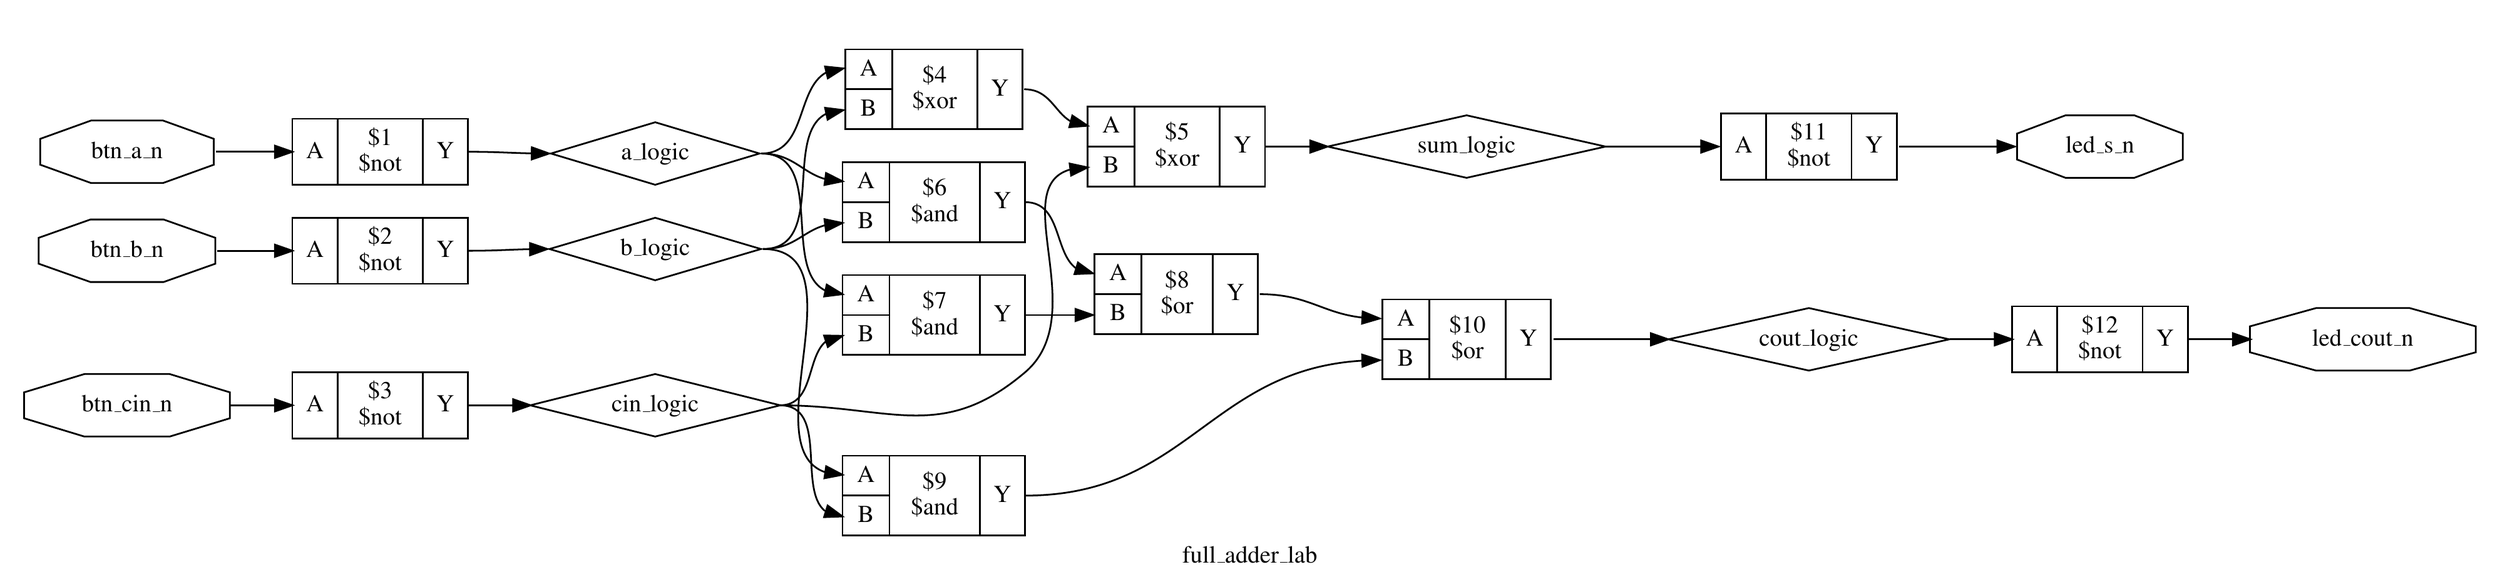
\begin{tikzpicture}[x=1bp,y=-1bp,line width=1bp,line cap=butt,line join=miter]
\path[draw=none,fill=white] (-4,4) -- (-4,-308) -- (1413.72,-308) -- (1413.72,4) -- cycle;
\node[anchor=base,inner sep=0pt,outer sep=0pt,text=black,font=\fontfamily{ptm}\fontsize{14.00bp}{14.00bp}\selectfont] at (704.86,-7.8) {full\_adder\_lab};
\path[draw=black,fill=none] (362.88,-261.5) -- (302.89,-243.5) -- (362.88,-225.5) -- (422.87,-243.5) -- cycle;
\node[anchor=base,inner sep=0pt,outer sep=0pt,text=black,font=\fontfamily{ptm}\fontsize{14.00bp}{14.00bp}\selectfont] at (362.88,-239.8) {a\_logic};
\path[draw=black,fill=none] (470.58,-192.5) -- (470.58,-238.5) -- (575.58,-238.5) -- (575.58,-192.5) -- cycle;
\node[anchor=base,inner sep=0pt,outer sep=0pt,text=black,font=\fontfamily{ptm}\fontsize{14.00bp}{14.00bp}\selectfont] at (484.08,-223.3) {A};
\path[draw=black,fill=none] (470.58,-215.5) -- (497.58,-215.5);
\node[anchor=base,inner sep=0pt,outer sep=0pt,text=black,font=\fontfamily{ptm}\fontsize{14.00bp}{14.00bp}\selectfont] at (484.08,-200.3) {B};
\path[draw=black,fill=none] (497.58,-192.5) -- (497.58,-238.5);
\node[anchor=base,inner sep=0pt,outer sep=0pt,text=black,font=\fontfamily{ptm}\fontsize{14.00bp}{14.00bp}\selectfont] at (523.58,-219.3) {\$6};
\node[anchor=base,inner sep=0pt,outer sep=0pt,text=black,font=\fontfamily{ptm}\fontsize{14.00bp}{14.00bp}\selectfont] at (523.58,-204.3) {\$and};
\path[draw=black,fill=none] (549.58,-192.5) -- (549.58,-238.5);
\node[anchor=base,inner sep=0pt,outer sep=0pt,text=black,font=\fontfamily{ptm}\fontsize{14.00bp}{14.00bp}\selectfont] at (562.58,-211.8) {Y};
\path[draw=black,fill=none] (423.88,-243.5) .. controls (441.88,-243.5) and (447.01,-232.73) .. (460.38,-228.86);
\path[draw=black,fill=black] (461.13,-232.3) -- (470.58,-227.5) -- (460.2,-225.36) -- cycle;
\path[draw=black,fill=none] (470.58,-127.5) -- (470.58,-173.5) -- (575.58,-173.5) -- (575.58,-127.5) -- cycle;
\node[anchor=base,inner sep=0pt,outer sep=0pt,text=black,font=\fontfamily{ptm}\fontsize{14.00bp}{14.00bp}\selectfont] at (484.08,-158.3) {A};
\path[draw=black,fill=none] (470.58,-150.5) -- (497.58,-150.5);
\node[anchor=base,inner sep=0pt,outer sep=0pt,text=black,font=\fontfamily{ptm}\fontsize{14.00bp}{14.00bp}\selectfont] at (484.08,-135.3) {B};
\path[draw=black,fill=none] (497.58,-127.5) -- (497.58,-173.5);
\node[anchor=base,inner sep=0pt,outer sep=0pt,text=black,font=\fontfamily{ptm}\fontsize{14.00bp}{14.00bp}\selectfont] at (523.58,-154.3) {\$7};
\node[anchor=base,inner sep=0pt,outer sep=0pt,text=black,font=\fontfamily{ptm}\fontsize{14.00bp}{14.00bp}\selectfont] at (523.58,-139.3) {\$and};
\path[draw=black,fill=none] (549.58,-127.5) -- (549.58,-173.5);
\node[anchor=base,inner sep=0pt,outer sep=0pt,text=black,font=\fontfamily{ptm}\fontsize{14.00bp}{14.00bp}\selectfont] at (562.58,-146.8) {Y};
\path[draw=black,fill=none] (423.88,-243.5) .. controls (461.38,-243.5) and (435.39,-177.55) .. (460.49,-164.67);
\path[draw=black,fill=black] (461.53,-168.02) -- (470.58,-162.5) -- (460.06,-161.18) -- cycle;
\path[draw=black,fill=none] (472.08,-257.5) -- (472.08,-303.5) -- (574.08,-303.5) -- (574.08,-257.5) -- cycle;
\node[anchor=base,inner sep=0pt,outer sep=0pt,text=black,font=\fontfamily{ptm}\fontsize{14.00bp}{14.00bp}\selectfont] at (485.58,-288.3) {A};
\path[draw=black,fill=none] (472.08,-280.5) -- (499.08,-280.5);
\node[anchor=base,inner sep=0pt,outer sep=0pt,text=black,font=\fontfamily{ptm}\fontsize{14.00bp}{14.00bp}\selectfont] at (485.58,-265.3) {B};
\path[draw=black,fill=none] (499.08,-257.5) -- (499.08,-303.5);
\node[anchor=base,inner sep=0pt,outer sep=0pt,text=black,font=\fontfamily{ptm}\fontsize{14.00bp}{14.00bp}\selectfont] at (523.58,-284.3) {\$4};
\node[anchor=base,inner sep=0pt,outer sep=0pt,text=black,font=\fontfamily{ptm}\fontsize{14.00bp}{14.00bp}\selectfont] at (523.58,-269.3) {\$xor};
\path[draw=black,fill=none] (548.08,-257.5) -- (548.08,-303.5);
\node[anchor=base,inner sep=0pt,outer sep=0pt,text=black,font=\fontfamily{ptm}\fontsize{14.00bp}{14.00bp}\selectfont] at (561.08,-276.8) {Y};
\path[draw=black,fill=none] (423.88,-243.5) .. controls (450.1,-243.5) and (443.6,-280.35) .. (461.13,-290.14);
\path[draw=black,fill=black] (460.54,-293.59) -- (471.08,-292.5) -- (462.16,-286.78) -- cycle;
\path[draw=black,fill=none] (362.88,-206.5) -- (302.05,-188.5) -- (362.88,-170.5) -- (423.71,-188.5) -- cycle;
\node[anchor=base,inner sep=0pt,outer sep=0pt,text=black,font=\fontfamily{ptm}\fontsize{14.00bp}{14.00bp}\selectfont] at (362.88,-184.8) {b\_logic};
\path[draw=black,fill=none] (424.88,-188.5) .. controls (442.42,-188.5) and (447.55,-198.59) .. (460.62,-202.22);
\path[draw=black,fill=black] (460.21,-205.7) -- (470.58,-203.5) -- (461.1,-198.75) -- cycle;
\path[draw=black,fill=none] (470.58,-23.5) -- (470.58,-69.5) -- (575.58,-69.5) -- (575.58,-23.5) -- cycle;
\node[anchor=base,inner sep=0pt,outer sep=0pt,text=black,font=\fontfamily{ptm}\fontsize{14.00bp}{14.00bp}\selectfont] at (484.08,-54.3) {A};
\path[draw=black,fill=none] (470.58,-46.5) -- (497.58,-46.5);
\node[anchor=base,inner sep=0pt,outer sep=0pt,text=black,font=\fontfamily{ptm}\fontsize{14.00bp}{14.00bp}\selectfont] at (484.08,-31.3) {B};
\path[draw=black,fill=none] (497.58,-23.5) -- (497.58,-69.5);
\node[anchor=base,inner sep=0pt,outer sep=0pt,text=black,font=\fontfamily{ptm}\fontsize{14.00bp}{14.00bp}\selectfont] at (523.58,-50.3) {\$9};
\node[anchor=base,inner sep=0pt,outer sep=0pt,text=black,font=\fontfamily{ptm}\fontsize{14.00bp}{14.00bp}\selectfont] at (523.58,-35.3) {\$and};
\path[draw=black,fill=none] (549.58,-23.5) -- (549.58,-69.5);
\node[anchor=base,inner sep=0pt,outer sep=0pt,text=black,font=\fontfamily{ptm}\fontsize{14.00bp}{14.00bp}\selectfont] at (562.58,-42.8) {Y};
\path[draw=black,fill=none] (424.88,-188.5) .. controls (482.3,-188.5) and (418.39,-74.24) .. (460.64,-59.96);
\path[draw=black,fill=black] (461.19,-63.42) -- (470.58,-58.5) -- (460.17,-56.49) -- cycle;
\path[draw=black,fill=none] (424.88,-188.5) .. controls (461.93,-188.5) and (436.3,-253.64) .. (461.11,-266.36);
\path[draw=black,fill=black] (460.56,-269.82) -- (471.08,-268.5) -- (462.03,-262.98) -- cycle;
\path[draw=black,fill=none] (108.99,-237.04) -- (108.99,-251.96) -- (79.76,-262.5) -- (38.43,-262.5) -- (9.2,-251.96) -- (9.2,-237.04) -- (38.43,-226.5) -- (79.76,-226.5) -- cycle;
\node[anchor=base,inner sep=0pt,outer sep=0pt,text=black,font=\fontfamily{ptm}\fontsize{14.00bp}{14.00bp}\selectfont] at (59.09,-240.8) {btn\_a\_n};
\path[draw=black,fill=none] (154.19,-225.5) -- (154.19,-263.5) -- (255.19,-263.5) -- (255.19,-225.5) -- cycle;
\node[anchor=base,inner sep=0pt,outer sep=0pt,text=black,font=\fontfamily{ptm}\fontsize{14.00bp}{14.00bp}\selectfont] at (167.19,-240.8) {A};
\path[draw=black,fill=none] (180.19,-225.5) -- (180.19,-263.5);
\node[anchor=base,inner sep=0pt,outer sep=0pt,text=black,font=\fontfamily{ptm}\fontsize{14.00bp}{14.00bp}\selectfont] at (204.69,-248.3) {\$1};
\node[anchor=base,inner sep=0pt,outer sep=0pt,text=black,font=\fontfamily{ptm}\fontsize{14.00bp}{14.00bp}\selectfont] at (204.69,-233.3) {\$not};
\path[draw=black,fill=none] (229.19,-225.5) -- (229.19,-263.5);
\node[anchor=base,inner sep=0pt,outer sep=0pt,text=black,font=\fontfamily{ptm}\fontsize{14.00bp}{14.00bp}\selectfont] at (242.19,-240.8) {Y};
\path[draw=black,fill=none] (110.09,-244.5) .. controls (125.86,-244.5) and (132.12,-244.5) .. (144.17,-244.5);
\path[draw=black,fill=black] (144.19,-248) -- (154.19,-244.5) -- (144.19,-241) -- cycle;
\path[draw=black,fill=none] (109.9,-180.04) -- (109.9,-194.96) -- (80.14,-205.5) -- (38.05,-205.5) -- (8.29,-194.96) -- (8.29,-180.04) -- (38.05,-169.5) -- (80.14,-169.5) -- cycle;
\node[anchor=base,inner sep=0pt,outer sep=0pt,text=black,font=\fontfamily{ptm}\fontsize{14.00bp}{14.00bp}\selectfont] at (59.09,-183.8) {btn\_b\_n};
\path[draw=black,fill=none] (154.19,-168.5) -- (154.19,-206.5) -- (255.19,-206.5) -- (255.19,-168.5) -- cycle;
\node[anchor=base,inner sep=0pt,outer sep=0pt,text=black,font=\fontfamily{ptm}\fontsize{14.00bp}{14.00bp}\selectfont] at (167.19,-183.8) {A};
\path[draw=black,fill=none] (180.19,-168.5) -- (180.19,-206.5);
\node[anchor=base,inner sep=0pt,outer sep=0pt,text=black,font=\fontfamily{ptm}\fontsize{14.00bp}{14.00bp}\selectfont] at (204.69,-191.3) {\$2};
\node[anchor=base,inner sep=0pt,outer sep=0pt,text=black,font=\fontfamily{ptm}\fontsize{14.00bp}{14.00bp}\selectfont] at (204.69,-176.3) {\$not};
\path[draw=black,fill=none] (229.19,-168.5) -- (229.19,-206.5);
\node[anchor=base,inner sep=0pt,outer sep=0pt,text=black,font=\fontfamily{ptm}\fontsize{14.00bp}{14.00bp}\selectfont] at (242.19,-183.8) {Y};
\path[draw=black,fill=none] (111.09,-187.5) .. controls (126.36,-187.5) and (132.5,-187.5) .. (144.05,-187.5);
\path[draw=black,fill=black] (144.19,-191) -- (154.19,-187.5) -- (144.19,-184) -- cycle;
\path[draw=black,fill=none] (118.28,-91.04) -- (118.28,-105.96) -- (83.61,-116.5) -- (34.58,-116.5) -- (-0.09,-105.96) -- (-0.09,-91.04) -- (34.58,-80.5) -- (83.61,-80.5) -- cycle;
\node[anchor=base,inner sep=0pt,outer sep=0pt,text=black,font=\fontfamily{ptm}\fontsize{14.00bp}{14.00bp}\selectfont] at (59.09,-94.8) {btn\_cin\_n};
\path[draw=black,fill=none] (154.19,-79.5) -- (154.19,-117.5) -- (255.19,-117.5) -- (255.19,-79.5) -- cycle;
\node[anchor=base,inner sep=0pt,outer sep=0pt,text=black,font=\fontfamily{ptm}\fontsize{14.00bp}{14.00bp}\selectfont] at (167.19,-94.8) {A};
\path[draw=black,fill=none] (180.19,-79.5) -- (180.19,-117.5);
\node[anchor=base,inner sep=0pt,outer sep=0pt,text=black,font=\fontfamily{ptm}\fontsize{14.00bp}{14.00bp}\selectfont] at (204.69,-102.3) {\$3};
\node[anchor=base,inner sep=0pt,outer sep=0pt,text=black,font=\fontfamily{ptm}\fontsize{14.00bp}{14.00bp}\selectfont] at (204.69,-87.3) {\$not};
\path[draw=black,fill=none] (229.19,-79.5) -- (229.19,-117.5);
\node[anchor=base,inner sep=0pt,outer sep=0pt,text=black,font=\fontfamily{ptm}\fontsize{14.00bp}{14.00bp}\selectfont] at (242.19,-94.8) {Y};
\path[draw=black,fill=none] (118.19,-98.5) .. controls (130.19,-98.5) and (135.44,-98.5) .. (144.06,-98.5);
\path[draw=black,fill=black] (144.19,-102) -- (154.19,-98.5) -- (144.19,-95) -- cycle;
\path[draw=black,fill=none] (362.88,-116.5) -- (290.99,-98.5) -- (362.88,-80.5) -- (434.77,-98.5) -- cycle;
\node[anchor=base,inner sep=0pt,outer sep=0pt,text=black,font=\fontfamily{ptm}\fontsize{14.00bp}{14.00bp}\selectfont] at (362.88,-94.8) {cin\_logic};
\path[draw=black,fill=none] (434.58,-98.5) .. controls (454.38,-98.5) and (449.67,-125.93) .. (461.05,-135.36);
\path[draw=black,fill=black] (459.98,-138.7) -- (470.58,-138.5) -- (462.17,-132.05) -- cycle;
\path[draw=black,fill=none] (434.58,-98.5) .. controls (462.88,-98.5) and (444.62,-50.37) .. (460.56,-37.59);
\path[draw=black,fill=black] (462.05,-40.79) -- (470.58,-34.5) -- (459.99,-34.1) -- cycle;
\path[draw=black,fill=none] (611.58,-224.5) -- (611.58,-270.5) -- (713.58,-270.5) -- (713.58,-224.5) -- cycle;
\node[anchor=base,inner sep=0pt,outer sep=0pt,text=black,font=\fontfamily{ptm}\fontsize{14.00bp}{14.00bp}\selectfont] at (625.08,-255.3) {A};
\path[draw=black,fill=none] (611.58,-247.5) -- (638.58,-247.5);
\node[anchor=base,inner sep=0pt,outer sep=0pt,text=black,font=\fontfamily{ptm}\fontsize{14.00bp}{14.00bp}\selectfont] at (625.08,-232.3) {B};
\path[draw=black,fill=none] (638.58,-224.5) -- (638.58,-270.5);
\node[anchor=base,inner sep=0pt,outer sep=0pt,text=black,font=\fontfamily{ptm}\fontsize{14.00bp}{14.00bp}\selectfont] at (663.08,-251.3) {\$5};
\node[anchor=base,inner sep=0pt,outer sep=0pt,text=black,font=\fontfamily{ptm}\fontsize{14.00bp}{14.00bp}\selectfont] at (663.08,-236.3) {\$xor};
\path[draw=black,fill=none] (687.58,-224.5) -- (687.58,-270.5);
\node[anchor=base,inner sep=0pt,outer sep=0pt,text=black,font=\fontfamily{ptm}\fontsize{14.00bp}{14.00bp}\selectfont] at (700.58,-243.8) {Y};
\path[draw=black,fill=none] (434.58,-98.5) .. controls (497.81,-98.5) and (527.39,-76.56) .. (575.58,-117.5) .. controls (614.26,-150.37) and (565.18,-223.51) .. (601.19,-234.19);
\path[draw=black,fill=black] (601.22,-237.72) -- (611.58,-235.5) -- (602.09,-230.78) -- cycle;
\path[draw=black,fill=none] (1026.39,-154.5) -- (945.62,-136.5) -- (1026.39,-118.5) -- (1107.17,-136.5) -- cycle;
\node[anchor=base,inner sep=0pt,outer sep=0pt,text=black,font=\fontfamily{ptm}\fontsize{14.00bp}{14.00bp}\selectfont] at (1026.39,-132.8) {cout\_logic};
\path[draw=black,fill=none] (1143.28,-117.5) -- (1143.28,-155.5) -- (1244.28,-155.5) -- (1244.28,-117.5) -- cycle;
\node[anchor=base,inner sep=0pt,outer sep=0pt,text=black,font=\fontfamily{ptm}\fontsize{14.00bp}{14.00bp}\selectfont] at (1156.28,-132.8) {A};
\path[draw=black,fill=none] (1169.28,-117.5) -- (1169.28,-155.5);
\node[anchor=base,inner sep=0pt,outer sep=0pt,text=black,font=\fontfamily{ptm}\fontsize{14.00bp}{14.00bp}\selectfont] at (1193.78,-140.3) {\$12};
\node[anchor=base,inner sep=0pt,outer sep=0pt,text=black,font=\fontfamily{ptm}\fontsize{14.00bp}{14.00bp}\selectfont] at (1193.78,-125.3) {\$not};
\path[draw=black,fill=none] (1218.28,-117.5) -- (1218.28,-155.5);
\node[anchor=base,inner sep=0pt,outer sep=0pt,text=black,font=\fontfamily{ptm}\fontsize{14.00bp}{14.00bp}\selectfont] at (1231.28,-132.8) {Y};
\path[draw=black,fill=none] (1107.28,-136.5) .. controls (1119.28,-136.5) and (1124.53,-136.5) .. (1133.16,-136.5);
\path[draw=black,fill=black] (1133.28,-140) -- (1143.28,-136.5) -- (1133.28,-133) -- cycle;
\path[draw=black,fill=none] (1409.95,-129.04) -- (1409.95,-143.96) -- (1371.9,-154.5) -- (1318.1,-154.5) -- (1280.06,-143.96) -- (1280.06,-129.04) -- (1318.1,-118.5) -- (1371.9,-118.5) -- cycle;
\node[anchor=base,inner sep=0pt,outer sep=0pt,text=black,font=\fontfamily{ptm}\fontsize{14.00bp}{14.00bp}\selectfont] at (1345,-132.8) {led\_cout\_n};
\path[draw=black,fill=none] (1241.46,-240.04) -- (1241.46,-254.96) -- (1213.53,-265.5) -- (1174.03,-265.5) -- (1146.1,-254.96) -- (1146.1,-240.04) -- (1174.03,-229.5) -- (1213.53,-229.5) -- cycle;
\node[anchor=base,inner sep=0pt,outer sep=0pt,text=black,font=\fontfamily{ptm}\fontsize{14.00bp}{14.00bp}\selectfont] at (1193.78,-243.8) {led\_s\_n};
\path[draw=black,fill=none] (829.54,-265.5) -- (749.61,-247.5) -- (829.54,-229.5) -- (909.48,-247.5) -- cycle;
\node[anchor=base,inner sep=0pt,outer sep=0pt,text=black,font=\fontfamily{ptm}\fontsize{14.00bp}{14.00bp}\selectfont] at (829.54,-243.8) {sum\_logic};
\path[draw=black,fill=none] (975.89,-228.5) -- (975.89,-266.5) -- (1076.89,-266.5) -- (1076.89,-228.5) -- cycle;
\node[anchor=base,inner sep=0pt,outer sep=0pt,text=black,font=\fontfamily{ptm}\fontsize{14.00bp}{14.00bp}\selectfont] at (988.89,-243.8) {A};
\path[draw=black,fill=none] (1001.89,-228.5) -- (1001.89,-266.5);
\node[anchor=base,inner sep=0pt,outer sep=0pt,text=black,font=\fontfamily{ptm}\fontsize{14.00bp}{14.00bp}\selectfont] at (1026.39,-251.3) {\$11};
\node[anchor=base,inner sep=0pt,outer sep=0pt,text=black,font=\fontfamily{ptm}\fontsize{14.00bp}{14.00bp}\selectfont] at (1026.39,-236.3) {\$not};
\path[draw=black,fill=none] (1050.89,-228.5) -- (1050.89,-266.5);
\node[anchor=base,inner sep=0pt,outer sep=0pt,text=black,font=\fontfamily{ptm}\fontsize{14.00bp}{14.00bp}\selectfont] at (1063.89,-243.8) {Y};
\path[draw=black,fill=none] (909.51,-247.5) .. controls (934.63,-247.5) and (943.34,-247.5) .. (964.23,-247.5);
\path[draw=black,fill=black] (964.39,-251) -- (974.39,-247.5) -- (964.39,-244) -- cycle;
\path[draw=black,fill=none] (615.58,-139.5) -- (615.58,-185.5) -- (709.58,-185.5) -- (709.58,-139.5) -- cycle;
\node[anchor=base,inner sep=0pt,outer sep=0pt,text=black,font=\fontfamily{ptm}\fontsize{14.00bp}{14.00bp}\selectfont] at (629.08,-170.3) {A};
\path[draw=black,fill=none] (615.58,-162.5) -- (642.58,-162.5);
\node[anchor=base,inner sep=0pt,outer sep=0pt,text=black,font=\fontfamily{ptm}\fontsize{14.00bp}{14.00bp}\selectfont] at (629.08,-147.3) {B};
\path[draw=black,fill=none] (642.58,-139.5) -- (642.58,-185.5);
\node[anchor=base,inner sep=0pt,outer sep=0pt,text=black,font=\fontfamily{ptm}\fontsize{14.00bp}{14.00bp}\selectfont] at (663.08,-166.3) {\$8};
\node[anchor=base,inner sep=0pt,outer sep=0pt,text=black,font=\fontfamily{ptm}\fontsize{14.00bp}{14.00bp}\selectfont] at (663.08,-151.3) {\$or};
\path[draw=black,fill=none] (683.58,-139.5) -- (683.58,-185.5);
\node[anchor=base,inner sep=0pt,outer sep=0pt,text=black,font=\fontfamily{ptm}\fontsize{14.00bp}{14.00bp}\selectfont] at (696.58,-158.8) {Y};
\path[draw=black,fill=none] (575.58,-215.5) .. controls (596.6,-215.5) and (592.15,-186.85) .. (604.82,-177.45);
\path[draw=black,fill=black] (606.02,-180.74) -- (614.58,-174.5) -- (603.99,-174.04) -- cycle;
\path[draw=black,fill=none] (575.58,-150.5) .. controls (588.98,-150.5) and (594.61,-150.5) .. (604.49,-150.5);
\path[draw=black,fill=black] (604.58,-154) -- (614.58,-150.5) -- (604.58,-147) -- cycle;
\path[draw=black,fill=none] (781.04,-113.5) -- (781.04,-159.5) -- (878.04,-159.5) -- (878.04,-113.5) -- cycle;
\node[anchor=base,inner sep=0pt,outer sep=0pt,text=black,font=\fontfamily{ptm}\fontsize{14.00bp}{14.00bp}\selectfont] at (794.54,-144.3) {A};
\path[draw=black,fill=none] (781.04,-136.5) -- (808.04,-136.5);
\node[anchor=base,inner sep=0pt,outer sep=0pt,text=black,font=\fontfamily{ptm}\fontsize{14.00bp}{14.00bp}\selectfont] at (794.54,-121.3) {B};
\path[draw=black,fill=none] (808.04,-113.5) -- (808.04,-159.5);
\node[anchor=base,inner sep=0pt,outer sep=0pt,text=black,font=\fontfamily{ptm}\fontsize{14.00bp}{14.00bp}\selectfont] at (830.04,-140.3) {\$10};
\node[anchor=base,inner sep=0pt,outer sep=0pt,text=black,font=\fontfamily{ptm}\fontsize{14.00bp}{14.00bp}\selectfont] at (830.04,-125.3) {\$or};
\path[draw=black,fill=none] (852.04,-113.5) -- (852.04,-159.5);
\node[anchor=base,inner sep=0pt,outer sep=0pt,text=black,font=\fontfamily{ptm}\fontsize{14.00bp}{14.00bp}\selectfont] at (865.04,-132.8) {Y};
\path[draw=black,fill=none] (575.58,-46.5) .. controls (669.12,-46.5) and (681.66,-118.97) .. (769.35,-124.2);
\path[draw=black,fill=black] (769.44,-127.71) -- (779.54,-124.5) -- (769.65,-120.71) -- cycle;
\path[draw=black,fill=none] (255.19,-244.5) .. controls (272.05,-244.5) and (278.63,-243.84) .. (291.64,-243.59);
\path[draw=black,fill=black] (291.91,-247.09) -- (301.88,-243.5) -- (291.85,-240.09) -- cycle;
\path[draw=black,fill=none] (255.19,-187.5) .. controls (271.69,-187.5) and (278.13,-188.16) .. (290.86,-188.41);
\path[draw=black,fill=black] (290.85,-191.91) -- (300.88,-188.5) -- (290.91,-184.91) -- cycle;
\path[draw=black,fill=none] (255.19,-98.5) .. controls (267.19,-98.5) and (272.44,-98.5) .. (281.06,-98.5);
\path[draw=black,fill=black] (281.19,-102) -- (291.19,-98.5) -- (281.19,-95) -- cycle;
\path[draw=black,fill=none] (1078.39,-247.5) .. controls (1104.21,-247.5) and (1113.09,-247.5) .. (1134.67,-247.5);
\path[draw=black,fill=black] (1134.78,-251) -- (1144.78,-247.5) -- (1134.78,-244) -- cycle;
\path[draw=black,fill=none] (1244.28,-136.5) .. controls (1256.28,-136.5) and (1261.53,-136.5) .. (1270.16,-136.5);
\path[draw=black,fill=black] (1270.28,-140) -- (1280.28,-136.5) -- (1270.28,-133) -- cycle;
\path[draw=black,fill=none] (879.54,-136.5) .. controls (905.2,-136.5) and (914.01,-136.5) .. (935.46,-136.5);
\path[draw=black,fill=black] (935.51,-140) -- (945.51,-136.5) -- (935.51,-133) -- cycle;
\path[draw=black,fill=none] (710.58,-162.5) .. controls (738.19,-162.5) and (746.42,-151.59) .. (769.49,-149.03);
\path[draw=black,fill=black] (769.74,-152.52) -- (779.54,-148.5) -- (769.37,-145.53) -- cycle;
\path[draw=black,fill=none] (575.08,-280.5) .. controls (589.7,-280.5) and (592.33,-267.68) .. (601.7,-262.08);
\path[draw=black,fill=black] (602.78,-265.41) -- (611.58,-259.5) -- (601.02,-258.64) -- cycle;
\path[draw=black,fill=none] (713.58,-247.5) .. controls (725.58,-247.5) and (730.83,-247.5) .. (739.45,-247.5);
\path[draw=black,fill=black] (739.58,-251) -- (749.58,-247.5) -- (739.58,-244) -- cycle;
\pgfresetboundingbox
\path[use as bounding box] (-4,4) rectangle (1413.72,-308);
\end{tikzpicture}

}\end{center}

{\small\raggedright Figure 1-1.3. Saved Yosys RTL view, before final generic gate mapping; SVG geometry converted to editable LaTeX vector paths.\par}

\begingroup\small\setlength{\tabcolsep}{4pt}
\renewcommand{\arraystretch}{1.20}
\noindent\begin{tabular}{@{}p{\dimexpr0.617647\linewidth-4.9412pt\relax}p{\dimexpr0.382353\linewidth-3.0588pt\relax}@{}}
\toprule
\textbf{Final Yosys metric} & \textbf{Value} \\
\midrule
Wires & 10 \\
Cells & 7 \\
Memories / processes & 0 / 0 \\
\bottomrule
\end{tabular}\par\endgroup
\vspace{2mm}

{\small\raggedright Table 1-1.4. Final generic synthesis statistics.\par}

{\small\raggedright Figure 1-1.3 shows the saved RTL structure before final generic gate mapping, and Table 1-1.4 summarizes the final generic synthesis statistics. For the input 011, summing the two 1s yields binary 10, which produces S=0 and Cout=1. With input 111, the calculation results in binary 11, so both outputs equal 1. It is critical to distinguish logical values from physical pin levels in this experiment: a logical 1 at the output corresponds to a pin level of 0 for the LED. Inverting both inputs and outputs aligns the button and LED states with the truth table. As expected for a combinational circuit, synthesis infers no latches or stored state.\par}

\clearpage

\section*{Lab 1-1 | Testing and results}

\subsection*{Verification method and testbench}

Inputs A, B and Cin were tested across all combinations from 000 to 111. As the full adder is a combinational circuit, these eight test cases fully cover its truth table. Outputs were verified after every input transition. The testbench defines input drivers as reg signals and output probes as wire signals. An initial block updates the input values every 10 ns. The input signals are inverted before being fed into the button ports, while LED outputs are inverted prior to comparison against expected values. The \texttt{\$dumpfile} and \texttt{\$dumpvars} commands store simulation waveforms in a VCD file. Expected outputs are directly computed from A+B+Cin: the sum modulo 2 yields S, and Cout equals 1 whenever the total sum is at least 2. This offers an independent verification of the XOR and carry expressions written in the design code. Table 1-1.5 compares expected and simulated outputs for all eight input combinations. LED pin levels have been converted back into logical values, and all eight results show perfect agreement.\par

\begingroup\small\setlength{\tabcolsep}{4pt}
\renewcommand{\arraystretch}{1.20}
\noindent\begin{tabular}{@{}p{\dimexpr0.235294\linewidth-5.6471pt\relax}p{\dimexpr0.276471\linewidth-6.6353pt\relax}p{\dimexpr0.276471\linewidth-6.6353pt\relax}p{\dimexpr0.211765\linewidth-5.0824pt\relax}@{}}
\toprule
\textbf{Logical inputs} & \textbf{Expected S, Cout} & \textbf{Actual S, Cout} & \textbf{Result} \\
\midrule
0 0 0 & 0 0 & 0 0 & PASS \\
0 0 1 & 1 0 & 1 0 & PASS \\
0 1 0 & 1 0 & 1 0 & PASS \\
0 1 1 & 0 1 & 0 1 & PASS \\
1 0 0 & 1 0 & 1 0 & PASS \\
1 0 1 & 0 1 & 0 1 & PASS \\
1 1 0 & 0 1 & 0 1 & PASS \\
1 1 1 & 1 1 & 1 1 & PASS \\
\bottomrule
\end{tabular}\par\endgroup
\vspace{2mm}

{\small\raggedright Table 1-1.5. Actual simulation results from the saved CSV.\par}

\subsection*{Waveform inspection and time analysis}

The saved VCD was visually inspected in GTKWave 3.3.116, with logical input/output signals and raw active-low pins. At a 40 ns marker, A=1, B=0 and Cin=0 gave S=1 and Cout=0; the raw LED pins were (0,1).\par

Figure 1-1.4 compares the expected logical outputs with the actual VCD outputs. They agree for every required truth-table interval. The figure is plotted from data; it is not a GTKWave screenshot.\par

These are ideal zero-delay functional results. The 10 ns spacing is the testbench observation interval, not a measured gate delay or hardware speed limit. Real propagation delay has not been measured.\par

\clearpage

\section*{Lab 1-1 | Waveform comparison}

\begin{center}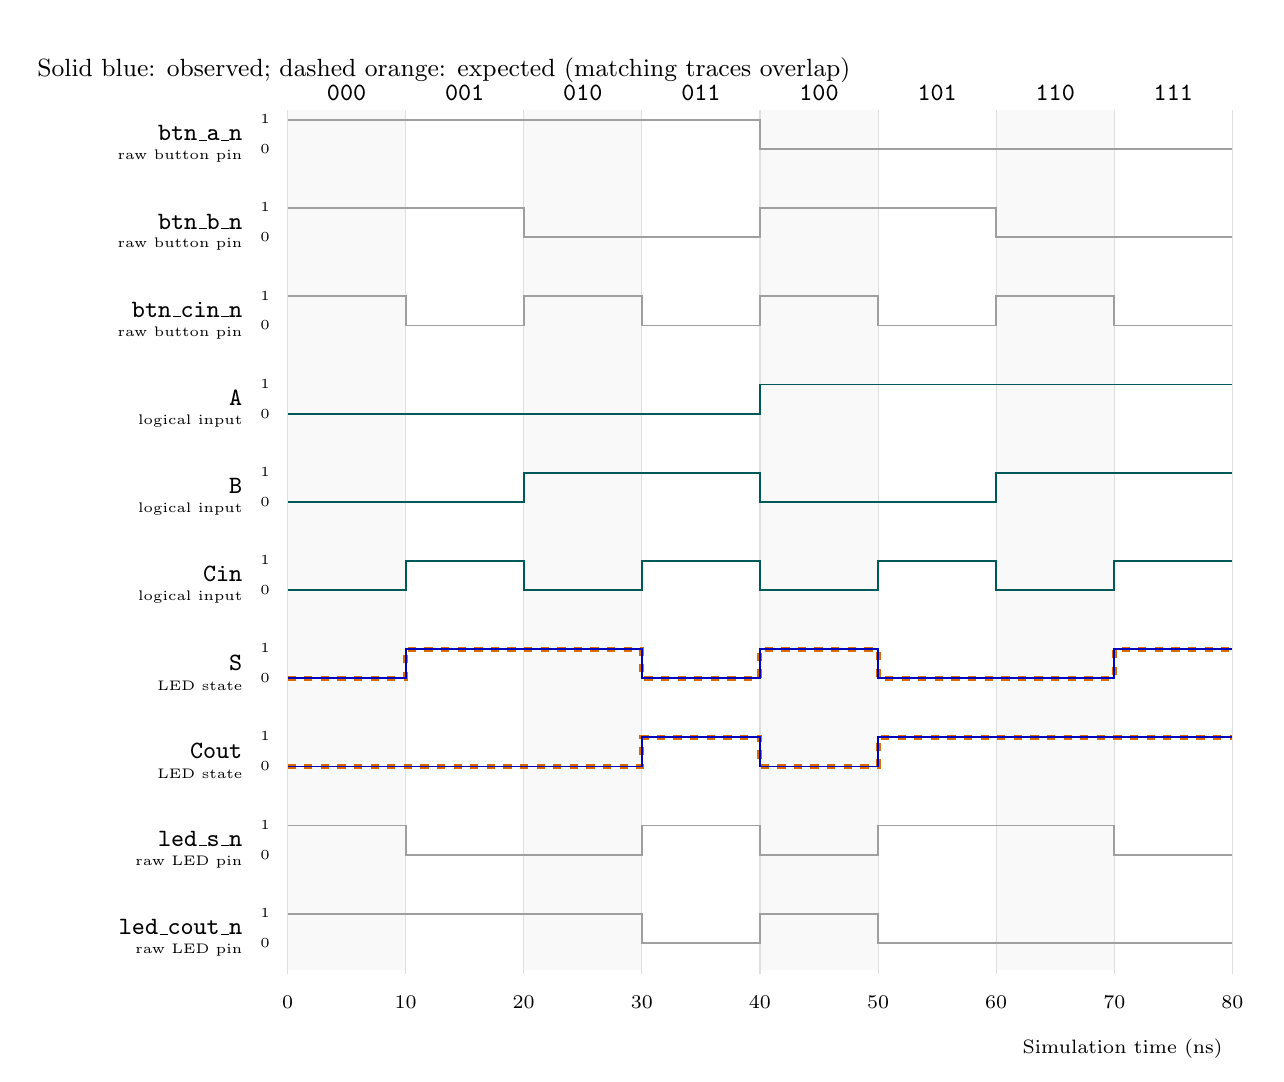
\begin{tikzpicture}[x=1cm,y=1cm,font=\scriptsize]
\path[use as bounding box] (-3.3,-1.1) rectangle (12.3,11.930000000000003);
\node[anchor=west,font=\small] at (-3.3,11.880000000000003) {Solid blue: observed; dashed orange: expected (matching traces overlap)};
\fill[gray!5] (0.0,.45) rectangle (1.5,11.380000000000003);
\node[font=\small\ttfamily] at (0.75,11.600000000000003) {000};
\node[font=\small\ttfamily] at (2.25,11.600000000000003) {001};
\fill[gray!5] (3.0,.45) rectangle (4.5,11.380000000000003);
\node[font=\small\ttfamily] at (3.75,11.600000000000003) {010};
\node[font=\small\ttfamily] at (5.25,11.600000000000003) {011};
\fill[gray!5] (6.0,.45) rectangle (7.5,11.380000000000003);
\node[font=\small\ttfamily] at (6.75,11.600000000000003) {100};
\node[font=\small\ttfamily] at (8.25,11.600000000000003) {101};
\fill[gray!5] (9.0,.45) rectangle (10.5,11.380000000000003);
\node[font=\small\ttfamily] at (9.75,11.600000000000003) {110};
\node[font=\small\ttfamily] at (11.25,11.600000000000003) {111};
\draw[gray!25] (0.0,.4) -- (0.0,11.380000000000003);
\node[below] at (0.0,.25) {0};
\draw[gray!25] (1.5,.4) -- (1.5,11.380000000000003);
\node[below] at (1.5,.25) {10};
\draw[gray!25] (3.0,.4) -- (3.0,11.380000000000003);
\node[below] at (3.0,.25) {20};
\draw[gray!25] (4.5,.4) -- (4.5,11.380000000000003);
\node[below] at (4.5,.25) {30};
\draw[gray!25] (6.0,.4) -- (6.0,11.380000000000003);
\node[below] at (6.0,.25) {40};
\draw[gray!25] (7.5,.4) -- (7.5,11.380000000000003);
\node[below] at (7.5,.25) {50};
\draw[gray!25] (9.0,.4) -- (9.0,11.380000000000003);
\node[below] at (9.0,.25) {60};
\draw[gray!25] (10.5,.4) -- (10.5,11.380000000000003);
\node[below] at (10.5,.25) {70};
\draw[gray!25] (12.0,.4) -- (12.0,11.380000000000003);
\node[below] at (12.0,.25) {80};
\node[anchor=east,font=\small\ttfamily] at (-.45,11.080000000000002) {btn\_a\_n};
\node[anchor=east,font=\tiny] at (-.45,10.790000000000003) {raw button pin};
\node[anchor=east,font=\tiny] at (-.1,11.260000000000003) {1};
\node[anchor=east,font=\tiny] at (-.1,10.880000000000003) {0};
\draw[gray!75,line width=.65pt] (0.0000,11.2500) -- (0.0000,11.2500) -- (0.0000,11.2500) -- (1.5000,11.2500) -- (1.5000,11.2500) -- (1.5000,11.2500) -- (3.0000,11.2500) -- (3.0000,11.2500) -- (3.0000,11.2500) -- (4.5000,11.2500) -- (4.5000,11.2500) -- (4.5000,11.2500) -- (6.0000,11.2500) -- (6.0000,11.2500) -- (6.0000,10.8800) -- (7.5000,10.8800) -- (7.5000,10.8800) -- (7.5000,10.8800) -- (9.0000,10.8800) -- (9.0000,10.8800) -- (9.0000,10.8800) -- (10.5000,10.8800) -- (10.5000,10.8800) -- (10.5000,10.8800) -- (12.0000,10.8800);
\node[anchor=east,font=\small\ttfamily] at (-.45,9.96) {btn\_b\_n};
\node[anchor=east,font=\tiny] at (-.45,9.670000000000002) {raw button pin};
\node[anchor=east,font=\tiny] at (-.1,10.140000000000002) {1};
\node[anchor=east,font=\tiny] at (-.1,9.760000000000002) {0};
\draw[gray!75,line width=.65pt] (0.0000,10.1300) -- (0.0000,10.1300) -- (0.0000,10.1300) -- (1.5000,10.1300) -- (1.5000,10.1300) -- (1.5000,10.1300) -- (3.0000,10.1300) -- (3.0000,10.1300) -- (3.0000,9.7600) -- (4.5000,9.7600) -- (4.5000,9.7600) -- (4.5000,9.7600) -- (6.0000,9.7600) -- (6.0000,9.7600) -- (6.0000,10.1300) -- (7.5000,10.1300) -- (7.5000,10.1300) -- (7.5000,10.1300) -- (9.0000,10.1300) -- (9.0000,10.1300) -- (9.0000,9.7600) -- (10.5000,9.7600) -- (10.5000,9.7600) -- (10.5000,9.7600) -- (12.0000,9.7600);
\node[anchor=east,font=\small\ttfamily] at (-.45,8.840000000000002) {btn\_cin\_n};
\node[anchor=east,font=\tiny] at (-.45,8.550000000000002) {raw button pin};
\node[anchor=east,font=\tiny] at (-.1,9.020000000000003) {1};
\node[anchor=east,font=\tiny] at (-.1,8.640000000000002) {0};
\draw[gray!75,line width=.65pt] (0.0000,9.0100) -- (0.0000,9.0100) -- (0.0000,9.0100) -- (1.5000,9.0100) -- (1.5000,9.0100) -- (1.5000,8.6400) -- (3.0000,8.6400) -- (3.0000,8.6400) -- (3.0000,9.0100) -- (4.5000,9.0100) -- (4.5000,9.0100) -- (4.5000,8.6400) -- (6.0000,8.6400) -- (6.0000,8.6400) -- (6.0000,9.0100) -- (7.5000,9.0100) -- (7.5000,9.0100) -- (7.5000,8.6400) -- (9.0000,8.6400) -- (9.0000,8.6400) -- (9.0000,9.0100) -- (10.5000,9.0100) -- (10.5000,9.0100) -- (10.5000,8.6400) -- (12.0000,8.6400);
\node[anchor=east,font=\small\ttfamily] at (-.45,7.720000000000002) {A};
\node[anchor=east,font=\tiny] at (-.45,7.430000000000002) {logical input};
\node[anchor=east,font=\tiny] at (-.1,7.900000000000002) {1};
\node[anchor=east,font=\tiny] at (-.1,7.520000000000002) {0};
\draw[teal!70!black,line width=.65pt] (0.0000,7.5200) -- (0.0000,7.5200) -- (0.0000,7.5200) -- (1.5000,7.5200) -- (1.5000,7.5200) -- (1.5000,7.5200) -- (3.0000,7.5200) -- (3.0000,7.5200) -- (3.0000,7.5200) -- (4.5000,7.5200) -- (4.5000,7.5200) -- (4.5000,7.5200) -- (6.0000,7.5200) -- (6.0000,7.5200) -- (6.0000,7.8900) -- (7.5000,7.8900) -- (7.5000,7.8900) -- (7.5000,7.8900) -- (9.0000,7.8900) -- (9.0000,7.8900) -- (9.0000,7.8900) -- (10.5000,7.8900) -- (10.5000,7.8900) -- (10.5000,7.8900) -- (12.0000,7.8900);
\node[anchor=east,font=\small\ttfamily] at (-.45,6.600000000000002) {B};
\node[anchor=east,font=\tiny] at (-.45,6.310000000000002) {logical input};
\node[anchor=east,font=\tiny] at (-.1,6.780000000000002) {1};
\node[anchor=east,font=\tiny] at (-.1,6.400000000000002) {0};
\draw[teal!70!black,line width=.65pt] (0.0000,6.4000) -- (0.0000,6.4000) -- (0.0000,6.4000) -- (1.5000,6.4000) -- (1.5000,6.4000) -- (1.5000,6.4000) -- (3.0000,6.4000) -- (3.0000,6.4000) -- (3.0000,6.7700) -- (4.5000,6.7700) -- (4.5000,6.7700) -- (4.5000,6.7700) -- (6.0000,6.7700) -- (6.0000,6.7700) -- (6.0000,6.4000) -- (7.5000,6.4000) -- (7.5000,6.4000) -- (7.5000,6.4000) -- (9.0000,6.4000) -- (9.0000,6.4000) -- (9.0000,6.7700) -- (10.5000,6.7700) -- (10.5000,6.7700) -- (10.5000,6.7700) -- (12.0000,6.7700);
\node[anchor=east,font=\small\ttfamily] at (-.45,5.480000000000002) {Cin};
\node[anchor=east,font=\tiny] at (-.45,5.190000000000002) {logical input};
\node[anchor=east,font=\tiny] at (-.1,5.660000000000002) {1};
\node[anchor=east,font=\tiny] at (-.1,5.280000000000002) {0};
\draw[teal!70!black,line width=.65pt] (0.0000,5.2800) -- (0.0000,5.2800) -- (0.0000,5.2800) -- (1.5000,5.2800) -- (1.5000,5.2800) -- (1.5000,5.6500) -- (3.0000,5.6500) -- (3.0000,5.6500) -- (3.0000,5.2800) -- (4.5000,5.2800) -- (4.5000,5.2800) -- (4.5000,5.6500) -- (6.0000,5.6500) -- (6.0000,5.6500) -- (6.0000,5.2800) -- (7.5000,5.2800) -- (7.5000,5.2800) -- (7.5000,5.6500) -- (9.0000,5.6500) -- (9.0000,5.6500) -- (9.0000,5.2800) -- (10.5000,5.2800) -- (10.5000,5.2800) -- (10.5000,5.6500) -- (12.0000,5.6500);
\node[anchor=east,font=\small\ttfamily] at (-.45,4.360000000000002) {S};
\node[anchor=east,font=\tiny] at (-.45,4.070000000000002) {LED state};
\node[anchor=east,font=\tiny] at (-.1,4.540000000000002) {1};
\node[anchor=east,font=\tiny] at (-.1,4.160000000000002) {0};
\draw[orange!85!black,line width=1.8pt,dashed] (0.0000,4.1600) -- (0.0000,4.1600) -- (0.0000,4.1600) -- (1.5000,4.1600) -- (1.5000,4.1600) -- (1.5000,4.5300) -- (3.0000,4.5300) -- (3.0000,4.5300) -- (3.0000,4.5300) -- (4.5000,4.5300) -- (4.5000,4.5300) -- (4.5000,4.1600) -- (6.0000,4.1600) -- (6.0000,4.1600) -- (6.0000,4.5300) -- (7.5000,4.5300) -- (7.5000,4.5300) -- (7.5000,4.1600) -- (9.0000,4.1600) -- (9.0000,4.1600) -- (9.0000,4.1600) -- (10.5000,4.1600) -- (10.5000,4.1600) -- (10.5000,4.5300) -- (12.0000,4.5300);
\draw[blue!75!black,line width=.65pt] (0.0000,4.1600) -- (0.0000,4.1600) -- (0.0000,4.1600) -- (1.5000,4.1600) -- (1.5000,4.1600) -- (1.5000,4.5300) -- (3.0000,4.5300) -- (3.0000,4.5300) -- (3.0000,4.5300) -- (4.5000,4.5300) -- (4.5000,4.5300) -- (4.5000,4.1600) -- (6.0000,4.1600) -- (6.0000,4.1600) -- (6.0000,4.5300) -- (7.5000,4.5300) -- (7.5000,4.5300) -- (7.5000,4.1600) -- (9.0000,4.1600) -- (9.0000,4.1600) -- (9.0000,4.1600) -- (10.5000,4.1600) -- (10.5000,4.1600) -- (10.5000,4.5300) -- (12.0000,4.5300);
\node[anchor=east,font=\small\ttfamily] at (-.45,3.240000000000002) {Cout};
\node[anchor=east,font=\tiny] at (-.45,2.950000000000002) {LED state};
\node[anchor=east,font=\tiny] at (-.1,3.4200000000000017) {1};
\node[anchor=east,font=\tiny] at (-.1,3.040000000000002) {0};
\draw[orange!85!black,line width=1.8pt,dashed] (0.0000,3.0400) -- (0.0000,3.0400) -- (0.0000,3.0400) -- (1.5000,3.0400) -- (1.5000,3.0400) -- (1.5000,3.0400) -- (3.0000,3.0400) -- (3.0000,3.0400) -- (3.0000,3.0400) -- (4.5000,3.0400) -- (4.5000,3.0400) -- (4.5000,3.4100) -- (6.0000,3.4100) -- (6.0000,3.4100) -- (6.0000,3.0400) -- (7.5000,3.0400) -- (7.5000,3.0400) -- (7.5000,3.4100) -- (9.0000,3.4100) -- (9.0000,3.4100) -- (9.0000,3.4100) -- (10.5000,3.4100) -- (10.5000,3.4100) -- (10.5000,3.4100) -- (12.0000,3.4100);
\draw[blue!75!black,line width=.65pt] (0.0000,3.0400) -- (0.0000,3.0400) -- (0.0000,3.0400) -- (1.5000,3.0400) -- (1.5000,3.0400) -- (1.5000,3.0400) -- (3.0000,3.0400) -- (3.0000,3.0400) -- (3.0000,3.0400) -- (4.5000,3.0400) -- (4.5000,3.0400) -- (4.5000,3.4100) -- (6.0000,3.4100) -- (6.0000,3.4100) -- (6.0000,3.0400) -- (7.5000,3.0400) -- (7.5000,3.0400) -- (7.5000,3.4100) -- (9.0000,3.4100) -- (9.0000,3.4100) -- (9.0000,3.4100) -- (10.5000,3.4100) -- (10.5000,3.4100) -- (10.5000,3.4100) -- (12.0000,3.4100);
\node[anchor=east,font=\small\ttfamily] at (-.45,2.120000000000002) {led\_s\_n};
\node[anchor=east,font=\tiny] at (-.45,1.8300000000000016) {raw LED pin};
\node[anchor=east,font=\tiny] at (-.1,2.3000000000000016) {1};
\node[anchor=east,font=\tiny] at (-.1,1.9200000000000017) {0};
\draw[gray!75,line width=.65pt] (0.0000,2.2900) -- (0.0000,2.2900) -- (0.0000,2.2900) -- (1.5000,2.2900) -- (1.5000,2.2900) -- (1.5000,1.9200) -- (3.0000,1.9200) -- (3.0000,1.9200) -- (3.0000,1.9200) -- (4.5000,1.9200) -- (4.5000,1.9200) -- (4.5000,2.2900) -- (6.0000,2.2900) -- (6.0000,2.2900) -- (6.0000,1.9200) -- (7.5000,1.9200) -- (7.5000,1.9200) -- (7.5000,2.2900) -- (9.0000,2.2900) -- (9.0000,2.2900) -- (9.0000,2.2900) -- (10.5000,2.2900) -- (10.5000,2.2900) -- (10.5000,1.9200) -- (12.0000,1.9200);
\node[anchor=east,font=\small\ttfamily] at (-.45,1.0000000000000007) {led\_cout\_n};
\node[anchor=east,font=\tiny] at (-.45,0.7100000000000007) {raw LED pin};
\node[anchor=east,font=\tiny] at (-.1,1.1800000000000006) {1};
\node[anchor=east,font=\tiny] at (-.1,0.8000000000000007) {0};
\draw[gray!75,line width=.65pt] (0.0000,1.1700) -- (0.0000,1.1700) -- (0.0000,1.1700) -- (1.5000,1.1700) -- (1.5000,1.1700) -- (1.5000,1.1700) -- (3.0000,1.1700) -- (3.0000,1.1700) -- (3.0000,1.1700) -- (4.5000,1.1700) -- (4.5000,1.1700) -- (4.5000,0.8000) -- (6.0000,0.8000) -- (6.0000,0.8000) -- (6.0000,1.1700) -- (7.5000,1.1700) -- (7.5000,1.1700) -- (7.5000,0.8000) -- (9.0000,0.8000) -- (9.0000,0.8000) -- (9.0000,0.8000) -- (10.5000,0.8000) -- (10.5000,0.8000) -- (10.5000,0.8000) -- (12.0000,0.8000);
\node[anchor=east] at (12,-.55) {Simulation time (ns)};
\end{tikzpicture}\end{center}
{\small All initial truth-table intervals agree. Logical signals: 1 = pressed/on; raw pins: 0 = pressed/on. The complete saved VCD contains 136 stable observations and zero disagreements. The plot shows settled interval values and does not resolve delta-cycle glitches.}\par

{\small\raggedright Figure 1-1.4. Actual VCD outputs and mathematical expectations; overlapping traces agree. Raw active-low pins are also shown.\par}

{\small\raggedright Logical signals use pressed/on = 1. Raw pins use pressed/on = 0. This comparison supports Table 1-1.5 and the active-low explanation in Table 1-1.2.\par}

\clearpage

\section*{Lab 1-1 | Board test and conclusion}

{\small\raggedright The mapped RTL was built with Verilator and displayed in the local SDL2 board window. The local input-support modification allows simultaneous states: keys 2 and 3 toggle B2 and B3; key 4 also toggles B4 for the adder; key 0 releases all inputs. This simulator adjustment does not change the task RTL [7].\par}

{\small\raggedright Table 1-1.6 records every visible case checked in the live window.\par}

\begingroup\small\setlength{\tabcolsep}{4pt}
\renewcommand{\arraystretch}{1.20}
\noindent\begin{tabular}{@{}p{\dimexpr0.205882\linewidth-3.2941pt\relax}p{\dimexpr0.558824\linewidth-8.9412pt\relax}p{\dimexpr0.235294\linewidth-3.7647pt\relax}@{}}
\toprule
\textbf{Logical inputs} & \textbf{Expected visible result} & \textbf{Observed} \\
\midrule
000 & S=0, Cout=0 & PASS \\
001 & S=1, Cout=0 & PASS \\
010 & S=1, Cout=0 & PASS \\
011 & S=0, Cout=1 & PASS \\
100 & S=1, Cout=0 & PASS \\
101 & S=0, Cout=1 & PASS \\
110 & S=0, Cout=1 & PASS \\
111 & S=1, Cout=1 & PASS \\
\bottomrule
\end{tabular}\par\endgroup
\vspace{2mm}

{\small\raggedright Table 1-1.6. Itemized virtual-board observations.\par}

{\small\raggedright Required public board-video link: \url{https://github.com/zhihanyu123/EIE330-Lab1-FullAdder-Comparator/blob/main/EIE330_Lab1_1_Full_Adder_Short.webm}.\par}

{\small\raggedright Local recording in the project bundle: full\_adder/evidence/full\_adder\_verified-screen0.webm\par}

{\small\raggedright Other board signals do not connect to the task module. The wrapper sets unused LEDs off and unused VGA outputs to inactive defaults.\par}

\subsection*{Discussion and conclusion}

{\small\raggedright The final full adder met all 8 required simulation and virtual-board cases. Yosys found no stored state. Simulation checks ideal Boolean behavior; generic synthesis does not establish fitted FPGA resources. These results validate the logic in software simulation and the virtual board. Physical FPGA operation and propagation delay were not measured.\par}

\subsection*{References}

{\small\raggedright [1] Macau University of Science and Technology, "EIE330 FPGA-based System Design - Lab 1 Requirements," course handout, accessed Oct. 8, 2026.\par}

{\small\raggedright [2] Macau University of Science and Technology, "EIE330 FPGA-based System Design: Lab 1-1 Simple LED Circuit," lecture slides, updated Oct. 5, 2026, accessed Oct. 8, 2026.\par}

{\small\raggedright [3] Altera Corporation, "Cyclone IV FPGA Device Family Overview," Cyclone IV Device Handbook, vol. 1, doc. CYIV-51001-2.0, Mar. 2016, Tables 1-1, 1-3 and Fig. 1-3.\par}

{\small\raggedright [4] Dongguan EmbedFire Electronic Technology Co., Ltd., "Wildfire EP4CE10 Pro schematic diagram," rev. V1.0, Sep. 14, 2023.\par}

{\small\raggedright [5] Icarus Verilog contributors, "Getting Started With Icarus Verilog." [Online]. Available: \url{https://steveicarus.github.io/iverilog/usage/getting_started.html}. Accessed: Oct. 8, 2026.\par}

{\small\raggedright [6] YosysHQ, "Synthesis starter." [Online]. Available: \url{https://yosyshq.readthedocs.io/projects/yosys/en/latest/getting_started/example_synth.html}. Accessed: Oct. 8, 2026.\par}

{\small\raggedright [7] pikipity, "Simple-VGA-Simulator," GitHub repository. [Online]. Available: \url{https://github.com/pikipity/Simple-VGA-Simulator}. Accessed: Oct. 8, 2026. Local input support is based on the saved source archive.\par}

{\small\raggedright [8] Massachusetts Institute of Technology, "Lectures 8/9," 6.111 Introductory Digital Systems Laboratory, Spring 2006, slides 5, 8. [Online]. Available: \url{https://web.mit.edu/6.111/www/s2006/LECTURES/l8_9.pdf}. Accessed: Oct. 8, 2026.\par}

\clearpage

\vspace*{65.1968503937008pt}

\section*{EIE330 FPGA-based System Design}

{\LARGE\bfseries Lab 1-2: One-bit Digital Comparator\par}\vspace{5mm}

Group 10 - three-member group\par

\vspace*{19.84251968503937pt}

\begingroup\small\setlength{\tabcolsep}{4pt}
\renewcommand{\arraystretch}{1.20}
\noindent\begin{tabular}{@{}p{\dimexpr0.117647\linewidth-1.8824pt\relax}p{\dimexpr0.529412\linewidth-8.4706pt\relax}p{\dimexpr0.352941\linewidth-5.6471pt\relax}@{}}
\toprule
\textbf{Member} & \textbf{Name} & \textbf{Student ID} \\
\midrule
1 & Yu Zhihan & 1240029016 \\
2 & Jiang Yaxi & 1240006481 \\
3 & Zhang Hankun & 1240006465 \\
\bottomrule
\end{tabular}\par\endgroup
\vspace{2mm}

{\small\raggedright Cover information for Lab 1-2.\par}

\subsection*{Experiment scope}

This report presents the full-adder and one-bit comparator experiments, including circuit design, implementation, functional simulation, virtual-board verification and results.\par

The recorded tests use software simulation and a virtual board. Physical FPGA confirmation has not been completed.\par

\clearpage

\section*{Lab 1-2 | Introduction and requirements}

A one-bit comparator shows whether A is less than, equal to or greater than B. Comparison is used in decision and control logic [8]. This circuit assigns the three relations to LED1, LED2 and LED3, respectively [1].\par

The aim is to implement this function using board buttons and LEDs. The design is one combinational module with active-low input and output pins. All 4 required truth-table cases matched the simulated expectations and all 4 visible virtual-board cases passed. Table 1-2.1 summarizes the hardware constraints.\par

\subsection*{Member contributions}

All three members participated in the complete workflow for both the full-adder and one-bit comparator experiments. Their shared work included requirements and datasheet review; circuit specifications, active-low interfaces and port mapping; truth tables, Boolean equations, block diagrams and expected-waveform review; RTL and testbench preparation; compilation, synthesis and RTL inspection; functional simulation, waveform comparison and simulation-time analysis; the required virtual-board cases and recordings; and report preparation, references, links and group review.\par

- Yu Zhihan (1240029016): participated in every stage of both experiments, from requirements and circuit design through implementation, testing and report preparation. Cross-checked the Boolean equations, RTL and active-low port mapping.\\
- Jiang Yaxi (1240006481): participated in every stage of both experiments, from requirements and circuit design through implementation, testing and report preparation. Cross-checked the testbench stimuli, expected outputs and simulation waveforms.\\
- Zhang Hankun (1240006465): participated in every stage of both experiments, from requirements and circuit design through implementation, testing and report preparation. Cross-checked the virtual-board observations, recordings, report figures, references and links.\par

\subsection*{AI use}

AI assistance was used for RTL/testbench drafting, verification and simulator input support, and report text/figures. All three members reviewed the AI-assisted material.\par

\subsection*{Group cross-check}

The three members cross-checked both circuits and compared the expected outputs with the simulation and virtual-board results. They checked all eight full-adder combinations and all four comparator combinations, then reviewed the consistency of the equations, RTL, interface polarity, waveforms, LED observations and report.\par

\subsection*{Design constraints}

\begingroup\small\setlength{\tabcolsep}{4pt}
\renewcommand{\arraystretch}{1.20}
\noindent\begin{tabular}{@{}p{\dimexpr0.176471\linewidth-1.4118pt\relax}p{\dimexpr0.823529\linewidth-6.5882pt\relax}@{}}
\toprule
\textbf{Item} & \textbf{Constraint} \\
\midrule
FPGA & Cyclone IV E EP4CE10F17C8N [2], [4] \\
Capacity & 10,320 logic elements; 179 user I/O pins in a 256-pin package [3] \\
Buttons & Released pin = 1, pressed pin = 0; nominal 3.3 V pull-up [2], [4] \\
LEDs & Pin 0 turns an LED on; pin 1 turns it off [1], [2] \\
Clock & Board clock is 50 MHz; this combinational circuit needs no clock or stored state [2] \\
\bottomrule
\end{tabular}\par\endgroup
\vspace{2mm}

{\small\raggedright Table 1-2.1. Hardware constraints used for the design.\par}

\clearpage

\section*{Lab 1-2 | Specification and system design}

Logical input 1 means pressed; logical output 1 means illuminated. Ports ending in \_n use the opposite pin value. Table 1-2.2 gives every port and its board-model connection [2]; Table 1-2.3 defines the complete function.\par

\begingroup\small\setlength{\tabcolsep}{4pt}
\renewcommand{\arraystretch}{1.20}
\noindent\begin{tabular}{@{}p{\dimexpr0.247059\linewidth-5.9294pt\relax}p{\dimexpr0.129412\linewidth-3.1059pt\relax}p{\dimexpr0.288235\linewidth-6.9176pt\relax}p{\dimexpr0.335294\linewidth-8.0471pt\relax}@{}}
\toprule
\textbf{Port (1 bit)} & \textbf{Direction} & \textbf{Active level} & \textbf{Board signal / label} \\
\midrule
btn\_a\_n & Input & 0 = A pressed & B2 / KEY1 \\
btn\_b\_n & Input & 0 = B pressed & B3 / KEY2 \\
led\_lt\_n & Output & 0 = LT LED on & led1 / LED0 \\
led\_eq\_n & Output & 0 = EQ LED on & led2 / LED1 \\
led\_gt\_n & Output & 0 = GT LED on & led3 / LED2 \\
\bottomrule
\end{tabular}\par\endgroup
\vspace{2mm}

{\small\raggedright Table 1-2.2. Ports of comparator\_lab and board-model mapping.\par}

\begingroup\small\setlength{\tabcolsep}{4pt}
\renewcommand{\arraystretch}{1.20}
\noindent\begin{tabular}{@{}p{\dimexpr0.441176\linewidth-3.5294pt\relax}p{\dimexpr0.558824\linewidth-4.4706pt\relax}@{}}
\toprule
\textbf{Logical inputs} & \textbf{Expected LT, EQ, GT} \\
\midrule
0 0 & 0 1 0 \\
0 1 & 1 0 0 \\
1 0 & 0 0 1 \\
1 1 & 0 1 0 \\
\bottomrule
\end{tabular}\par\endgroup
\vspace{2mm}

{\small\raggedright Table 1-2.3. Complete required truth table; output 1 means LED on.\par}

Figure 1-2.1 labels the structure and all signals. No other board input connects to the task module.\par

\begin{center}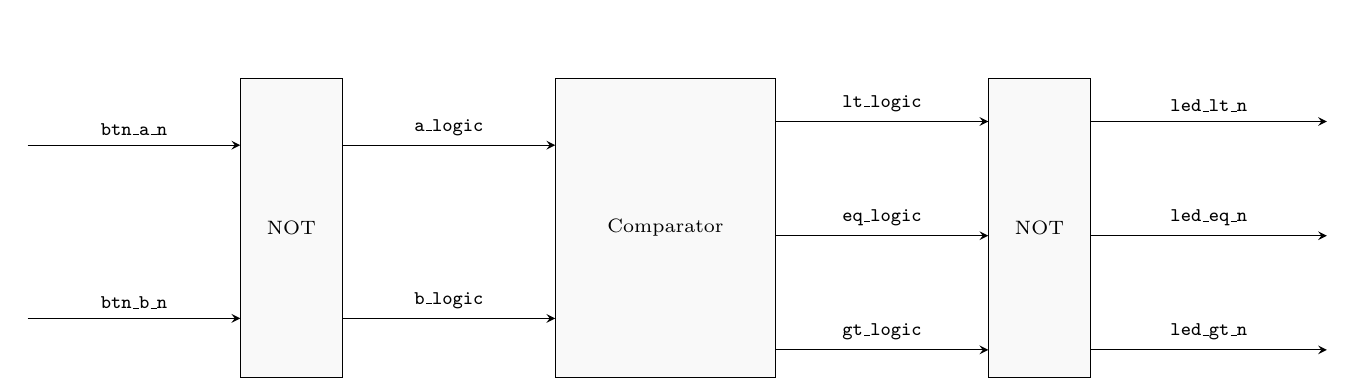
\begin{tikzpicture}[x=1cm,y=1cm,>=stealth,font=\scriptsize]
\path[use as bounding box] (0,0) rectangle (16.5,4.2);
\draw[fill=gray!5] (2.7,.25) rectangle (4.0,4.05);
\node at (3.35,2.15) {NOT};
\draw[fill=gray!5] (6.7,.25) rectangle (9.5,4.05);
\node at (8.1,2.15) {Comparator};
\draw[fill=gray!5] (12.2,.25) rectangle (13.5,4.05);
\node at (12.85,2.15) {NOT};
\draw[->] (0,3.2) -- (2.7,3.2);
\node[above] at (1.35,3.2) {\texttt{btn\_a\_n}};
\draw[->] (4,3.2) -- (6.7,3.2);
\node[above] at (5.35,3.2) {\texttt{a\_logic}};
\draw[->] (0,1) -- (2.7,1);
\node[above] at (1.35,1) {\texttt{btn\_b\_n}};
\draw[->] (4,1) -- (6.7,1);
\node[above] at (5.35,1) {\texttt{b\_logic}};
\draw[->] (9.5,3.5) -- (12.2,3.5);
\node[above] at (10.85,3.5) {\texttt{lt\_logic}};
\draw[->] (13.5,3.5) -- (16.5,3.5);
\node[above] at (15.0,3.5) {\texttt{led\_lt\_n}};
\draw[->] (9.5,2.05) -- (12.2,2.05);
\node[above] at (10.85,2.05) {\texttt{eq\_logic}};
\draw[->] (13.5,2.05) -- (16.5,2.05);
\node[above] at (15.0,2.05) {\texttt{led\_eq\_n}};
\draw[->] (9.5,0.6) -- (12.2,0.6);
\node[above] at (10.85,0.6) {\texttt{gt\_logic}};
\draw[->] (13.5,0.6) -- (16.5,0.6);
\node[above] at (15.0,0.6) {\texttt{led\_gt\_n}};
\end{tikzpicture}\end{center}

{\small\raggedright Figure 1-2.1. Input inversion, combinational logic and output inversion.\par}

The equations are LT = (NOT A) AND B, EQ = NOT (A XOR B), and GT = A AND (NOT B). Exactly one relation is true for any valid input pair.\par

Continuous dataflow assignments are suitable because the outputs depend only on the current inputs. One module is sufficient for this small circuit. Input and output inversion satisfy the active-low board interface.\par

Traceability: the port table defines input/output polarity; the truth table defines the function; the block diagram implements it. The simulation rows and board checklist test the same cases.\par

\clearpage

\section*{Lab 1-2 | Implementation}

Figure 1-2.2 gives the expected initial sequence, holding each case for 10 ns. It is a report reference reconstructed from the truth table, not a preserved pre-coding student drawing.\par

\begin{center}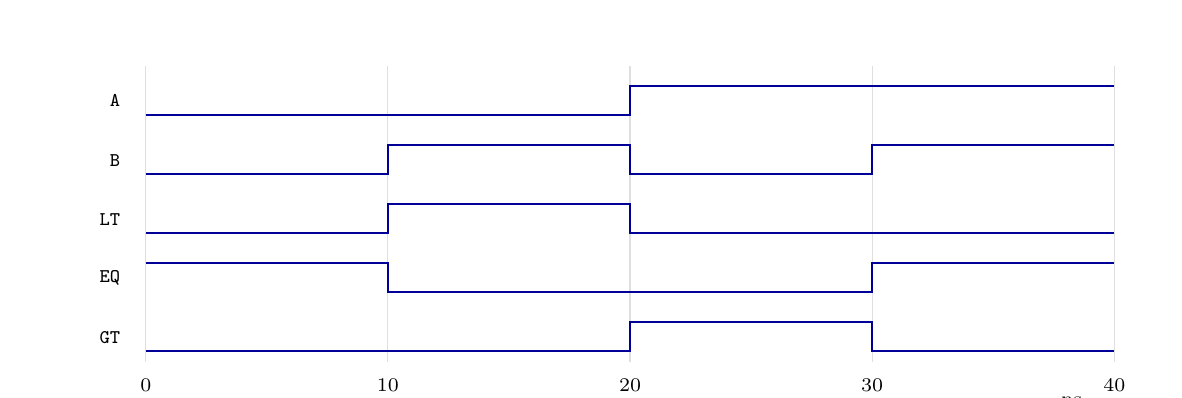
\begin{tikzpicture}[x=1cm,y=1cm,font=\scriptsize]
\path[use as bounding box] (-1.5,-.6) rectangle (12.8,3.75);
\draw[gray!25] (0.0,0) -- (0.0,3.75);
\node[below] at (0.0,-.1) {0};
\draw[gray!25] (3.075,0) -- (3.075,3.75);
\node[below] at (3.075,-.1) {10};
\draw[gray!25] (6.15,0) -- (6.15,3.75);
\node[below] at (6.15,-.1) {20};
\draw[gray!25] (9.225000000000001,0) -- (9.225000000000001,3.75);
\node[below] at (9.225000000000001,-.1) {30};
\draw[gray!25] (12.3,0) -- (12.3,3.75);
\node[below] at (12.3,-.1) {40};
\node[anchor=east] at (-.2,3.31) {\texttt{A}};
\draw[blue!60!black,line width=.7pt] (0.0000,3.1300) -- (0.0000,3.1300) -- (0.0000,3.1300) -- (3.0750,3.1300) -- (3.0750,3.1300) -- (3.0750,3.1300) -- (6.1500,3.1300) -- (6.1500,3.1300) -- (6.1500,3.5000) -- (9.2250,3.5000) -- (9.2250,3.5000) -- (9.2250,3.5000) -- (12.3000,3.5000);
\node[anchor=east] at (-.2,2.56) {\texttt{B}};
\draw[blue!60!black,line width=.7pt] (0.0000,2.3800) -- (0.0000,2.3800) -- (0.0000,2.3800) -- (3.0750,2.3800) -- (3.0750,2.3800) -- (3.0750,2.7500) -- (6.1500,2.7500) -- (6.1500,2.7500) -- (6.1500,2.3800) -- (9.2250,2.3800) -- (9.2250,2.3800) -- (9.2250,2.7500) -- (12.3000,2.7500);
\node[anchor=east] at (-.2,1.8099999999999998) {\texttt{LT}};
\draw[blue!60!black,line width=.7pt] (0.0000,1.6300) -- (0.0000,1.6300) -- (0.0000,1.6300) -- (3.0750,1.6300) -- (3.0750,1.6300) -- (3.0750,2.0000) -- (6.1500,2.0000) -- (6.1500,2.0000) -- (6.1500,1.6300) -- (9.2250,1.6300) -- (9.2250,1.6300) -- (9.2250,1.6300) -- (12.3000,1.6300);
\node[anchor=east] at (-.2,1.06) {\texttt{EQ}};
\draw[blue!60!black,line width=.7pt] (0.0000,1.2500) -- (0.0000,1.2500) -- (0.0000,1.2500) -- (3.0750,1.2500) -- (3.0750,1.2500) -- (3.0750,0.8800) -- (6.1500,0.8800) -- (6.1500,0.8800) -- (6.1500,0.8800) -- (9.2250,0.8800) -- (9.2250,0.8800) -- (9.2250,1.2500) -- (12.3000,1.2500);
\node[anchor=east] at (-.2,0.31) {\texttt{GT}};
\draw[blue!60!black,line width=.7pt] (0.0000,0.1300) -- (0.0000,0.1300) -- (0.0000,0.1300) -- (3.0750,0.1300) -- (3.0750,0.1300) -- (3.0750,0.1300) -- (6.1500,0.1300) -- (6.1500,0.1300) -- (6.1500,0.5000) -- (9.2250,0.5000) -- (9.2250,0.5000) -- (9.2250,0.1300) -- (12.3000,0.1300);
\node[anchor=west] at (11.5,-.5) {ns};
\end{tikzpicture}\end{center}

{\small\raggedright Figure 1-2.2. Expected logical input/output waveforms.\par}

The design is stored in RTL/ and the testbench in sim/ in the project bundle. A short implementation excerpt is shown below. The course requires publishing the complete RTL and testbench through GitHub [1].\par

\begin{verbatim}
assign eq_logic = ~(a_logic ^ b_logic);
assign led_eq_n = ~eq_logic;
\end{verbatim}

{\small\raggedright Project repository for RTL and testbench: \url{https://github.com/zhihanyu123/EIE330-Lab1-FullAdder-Comparator}. The repository currently hosts the verification videos and an earlier report copy. The full RTL and testbench are included in the local project bundle; their upload to this repository remains outstanding [1].\par}

{\small\raggedright Icarus Verilog 12.0 compiled cleanly. Yosys 0.33 reported no warnings and zero check problems. The final run compiled the design, checked and synthesized it, then executed functional simulation [5], [6].\par}

\begin{center}\resizebox{\linewidth}{!}{%
% Converted from preserved comparator/evidence/rtl.svg (Graphviz/Yosys RTL view).
% SHA-256: ea38b783d4fc4911481c984c62ee211def22c42578a5b55d0af1ea538a85c375
% All paths/arrowheads/shape vertices and text positions retain SVG coordinates.
% Text is editable Times-family TeX text; glyph metrics may differ slightly from SVG.
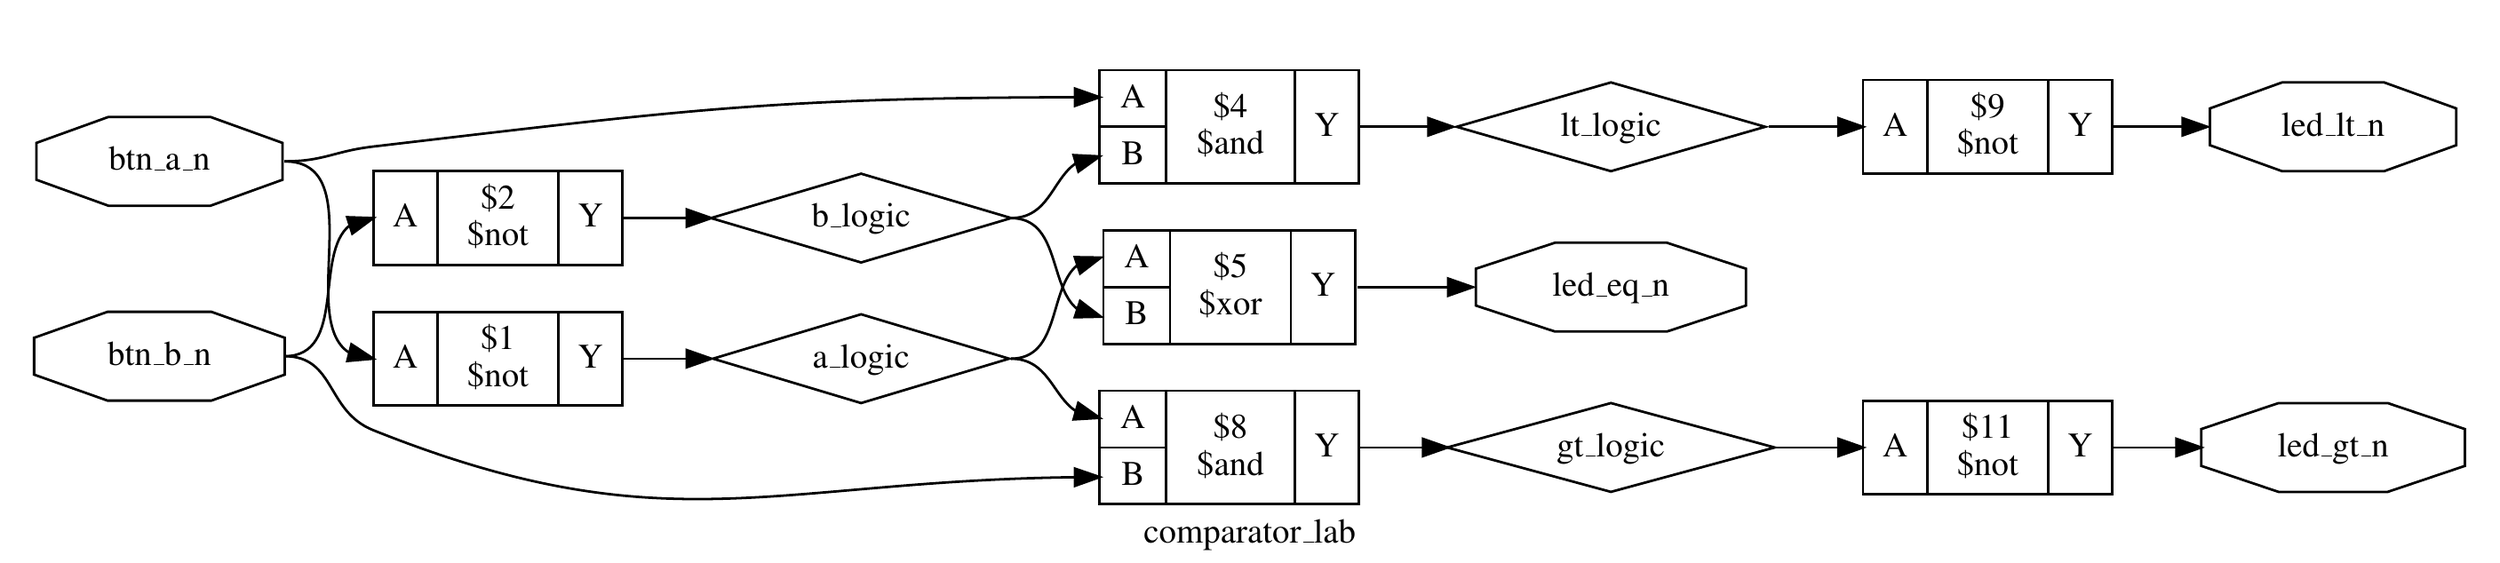
\begin{tikzpicture}[x=1bp,y=-1bp,line width=1bp,line cap=butt,line join=miter]
\path[draw=none,fill=white] (-4,4) -- (-4,-204) -- (988.92,-204) -- (988.92,4) -- cycle;
\node[anchor=base,inner sep=0pt,outer sep=0pt,text=black,font=\fontfamily{ptm}\fontsize{14.00bp}{14.00bp}\selectfont] at (492.46,-7.8) {comparator\_lab};
\path[draw=black,fill=none] (334.97,-100.5) -- (274.98,-82.5) -- (334.97,-64.5) -- (394.96,-82.5) -- cycle;
\node[anchor=base,inner sep=0pt,outer sep=0pt,text=black,font=\fontfamily{ptm}\fontsize{14.00bp}{14.00bp}\selectfont] at (334.97,-78.8) {a\_logic};
\path[draw=black,fill=none] (431.63,-23.5) -- (431.63,-69.5) -- (536.63,-69.5) -- (536.63,-23.5) -- cycle;
\node[anchor=base,inner sep=0pt,outer sep=0pt,text=black,font=\fontfamily{ptm}\fontsize{14.00bp}{14.00bp}\selectfont] at (445.13,-54.3) {A};
\path[draw=black,fill=none] (431.63,-46.5) -- (458.63,-46.5);
\node[anchor=base,inner sep=0pt,outer sep=0pt,text=black,font=\fontfamily{ptm}\fontsize{14.00bp}{14.00bp}\selectfont] at (445.13,-31.3) {B};
\path[draw=black,fill=none] (458.63,-23.5) -- (458.63,-69.5);
\node[anchor=base,inner sep=0pt,outer sep=0pt,text=black,font=\fontfamily{ptm}\fontsize{14.00bp}{14.00bp}\selectfont] at (484.63,-50.3) {\$8};
\node[anchor=base,inner sep=0pt,outer sep=0pt,text=black,font=\fontfamily{ptm}\fontsize{14.00bp}{14.00bp}\selectfont] at (484.63,-35.3) {\$and};
\path[draw=black,fill=none] (510.63,-23.5) -- (510.63,-69.5);
\node[anchor=base,inner sep=0pt,outer sep=0pt,text=black,font=\fontfamily{ptm}\fontsize{14.00bp}{14.00bp}\selectfont] at (523.63,-42.8) {Y};
\path[draw=black,fill=none] (395.63,-82.5) .. controls (410.81,-82.5) and (412.47,-67.56) .. (421.95,-61.25);
\path[draw=black,fill=black] (422.97,-64.6) -- (431.63,-58.5) -- (421.06,-57.87) -- cycle;
\path[draw=black,fill=none] (433.13,-88.5) -- (433.13,-134.5) -- (535.13,-134.5) -- (535.13,-88.5) -- cycle;
\node[anchor=base,inner sep=0pt,outer sep=0pt,text=black,font=\fontfamily{ptm}\fontsize{14.00bp}{14.00bp}\selectfont] at (446.63,-119.3) {A};
\path[draw=black,fill=none] (433.13,-111.5) -- (460.13,-111.5);
\node[anchor=base,inner sep=0pt,outer sep=0pt,text=black,font=\fontfamily{ptm}\fontsize{14.00bp}{14.00bp}\selectfont] at (446.63,-96.3) {B};
\path[draw=black,fill=none] (460.13,-88.5) -- (460.13,-134.5);
\node[anchor=base,inner sep=0pt,outer sep=0pt,text=black,font=\fontfamily{ptm}\fontsize{14.00bp}{14.00bp}\selectfont] at (484.63,-115.3) {\$5};
\node[anchor=base,inner sep=0pt,outer sep=0pt,text=black,font=\fontfamily{ptm}\fontsize{14.00bp}{14.00bp}\selectfont] at (484.63,-100.3) {\$xor};
\path[draw=black,fill=none] (509.13,-88.5) -- (509.13,-134.5);
\node[anchor=base,inner sep=0pt,outer sep=0pt,text=black,font=\fontfamily{ptm}\fontsize{14.00bp}{14.00bp}\selectfont] at (522.13,-107.8) {Y};
\path[draw=black,fill=none] (395.63,-82.5) .. controls (415.84,-82.5) and (410.88,-110.62) .. (422.43,-120.28);
\path[draw=black,fill=black] (421.54,-123.67) -- (432.13,-123.5) -- (423.74,-117.03) -- cycle;
\path[draw=black,fill=none] (334.97,-157.5) -- (274.14,-139.5) -- (334.97,-121.5) -- (395.8,-139.5) -- cycle;
\node[anchor=base,inner sep=0pt,outer sep=0pt,text=black,font=\fontfamily{ptm}\fontsize{14.00bp}{14.00bp}\selectfont] at (334.97,-135.8) {b\_logic};
\path[draw=black,fill=none] (431.63,-153.5) -- (431.63,-199.5) -- (536.63,-199.5) -- (536.63,-153.5) -- cycle;
\node[anchor=base,inner sep=0pt,outer sep=0pt,text=black,font=\fontfamily{ptm}\fontsize{14.00bp}{14.00bp}\selectfont] at (445.13,-184.3) {A};
\path[draw=black,fill=none] (431.63,-176.5) -- (458.63,-176.5);
\node[anchor=base,inner sep=0pt,outer sep=0pt,text=black,font=\fontfamily{ptm}\fontsize{14.00bp}{14.00bp}\selectfont] at (445.13,-161.3) {B};
\path[draw=black,fill=none] (458.63,-153.5) -- (458.63,-199.5);
\node[anchor=base,inner sep=0pt,outer sep=0pt,text=black,font=\fontfamily{ptm}\fontsize{14.00bp}{14.00bp}\selectfont] at (484.63,-180.3) {\$4};
\node[anchor=base,inner sep=0pt,outer sep=0pt,text=black,font=\fontfamily{ptm}\fontsize{14.00bp}{14.00bp}\selectfont] at (484.63,-165.3) {\$and};
\path[draw=black,fill=none] (510.63,-153.5) -- (510.63,-199.5);
\node[anchor=base,inner sep=0pt,outer sep=0pt,text=black,font=\fontfamily{ptm}\fontsize{14.00bp}{14.00bp}\selectfont] at (523.63,-172.8) {Y};
\path[draw=black,fill=none] (395.63,-139.5) .. controls (411,-139.5) and (412.4,-155.07) .. (421.88,-161.63);
\path[draw=black,fill=black] (421.05,-165.04) -- (431.63,-164.5) -- (423.03,-158.32) -- cycle;
\path[draw=black,fill=none] (395.63,-139.5) .. controls (415.56,-139.5) and (411.01,-112.07) .. (422.52,-102.64);
\path[draw=black,fill=black] (423.71,-105.93) -- (432.13,-99.5) -- (421.54,-99.28) -- cycle;
\path[draw=black,fill=none] (100.55,-155.04) -- (100.55,-169.96) -- (71.32,-180.5) -- (29.98,-180.5) -- (0.76,-169.96) -- (0.76,-155.04) -- (29.98,-144.5) -- (71.32,-144.5) -- cycle;
\node[anchor=base,inner sep=0pt,outer sep=0pt,text=black,font=\fontfamily{ptm}\fontsize{14.00bp}{14.00bp}\selectfont] at (50.65,-158.8) {btn\_a\_n};
\path[draw=black,fill=none] (101.3,-162.5) .. controls (117.52,-162.5) and (121.19,-166.61) .. (137.3,-168.5) .. controls (264.09,-183.34) and (298.71,-188.24) .. (421.46,-188.49);
\path[draw=black,fill=black] (421.63,-191.99) -- (431.63,-188.5) -- (421.64,-184.99) -- cycle;
\path[draw=black,fill=none] (137.3,-63.5) -- (137.3,-101.5) -- (238.3,-101.5) -- (238.3,-63.5) -- cycle;
\node[anchor=base,inner sep=0pt,outer sep=0pt,text=black,font=\fontfamily{ptm}\fontsize{14.00bp}{14.00bp}\selectfont] at (150.3,-78.8) {A};
\path[draw=black,fill=none] (163.3,-63.5) -- (163.3,-101.5);
\node[anchor=base,inner sep=0pt,outer sep=0pt,text=black,font=\fontfamily{ptm}\fontsize{14.00bp}{14.00bp}\selectfont] at (187.8,-86.3) {\$1};
\node[anchor=base,inner sep=0pt,outer sep=0pt,text=black,font=\fontfamily{ptm}\fontsize{14.00bp}{14.00bp}\selectfont] at (187.8,-71.3) {\$not};
\path[draw=black,fill=none] (212.3,-63.5) -- (212.3,-101.5);
\node[anchor=base,inner sep=0pt,outer sep=0pt,text=black,font=\fontfamily{ptm}\fontsize{14.00bp}{14.00bp}\selectfont] at (225.3,-78.8) {Y};
\path[draw=black,fill=none] (101.3,-162.5) .. controls (136.18,-162.5) and (106.27,-98.49) .. (127.48,-84.98);
\path[draw=black,fill=black] (128.46,-88.34) -- (137.3,-82.5) -- (126.75,-81.56) -- cycle;
\path[draw=black,fill=none] (101.45,-76.04) -- (101.45,-90.96) -- (71.69,-101.5) -- (29.61,-101.5) -- (-0.15,-90.96) -- (-0.15,-76.04) -- (29.61,-65.5) -- (71.69,-65.5) -- cycle;
\node[anchor=base,inner sep=0pt,outer sep=0pt,text=black,font=\fontfamily{ptm}\fontsize{14.00bp}{14.00bp}\selectfont] at (50.65,-79.8) {btn\_b\_n};
\path[draw=black,fill=none] (101.3,-83.5) .. controls (122.13,-83.5) and (117.96,-61.22) .. (137.3,-53.5) .. controls (255.85,-6.21) and (298.3,-32.99) .. (421.45,-34.44);
\path[draw=black,fill=black] (421.61,-37.94) -- (431.63,-34.5) -- (421.65,-30.94) -- cycle;
\path[draw=black,fill=none] (137.3,-120.5) -- (137.3,-158.5) -- (238.3,-158.5) -- (238.3,-120.5) -- cycle;
\node[anchor=base,inner sep=0pt,outer sep=0pt,text=black,font=\fontfamily{ptm}\fontsize{14.00bp}{14.00bp}\selectfont] at (150.3,-135.8) {A};
\path[draw=black,fill=none] (163.3,-120.5) -- (163.3,-158.5);
\node[anchor=base,inner sep=0pt,outer sep=0pt,text=black,font=\fontfamily{ptm}\fontsize{14.00bp}{14.00bp}\selectfont] at (187.8,-143.3) {\$2};
\node[anchor=base,inner sep=0pt,outer sep=0pt,text=black,font=\fontfamily{ptm}\fontsize{14.00bp}{14.00bp}\selectfont] at (187.8,-128.3) {\$not};
\path[draw=black,fill=none] (212.3,-120.5) -- (212.3,-158.5);
\node[anchor=base,inner sep=0pt,outer sep=0pt,text=black,font=\fontfamily{ptm}\fontsize{14.00bp}{14.00bp}\selectfont] at (225.3,-135.8) {Y};
\path[draw=black,fill=none] (101.3,-83.5) .. controls (126.73,-83.5) and (113.19,-124.86) .. (127.66,-136.49);
\path[draw=black,fill=black] (126.71,-139.86) -- (137.3,-139.5) -- (128.8,-133.18) -- cycle;
\path[draw=black,fill=none] (638.81,-64.5) -- (572.45,-46.5) -- (638.81,-28.5) -- (705.17,-46.5) -- cycle;
\node[anchor=base,inner sep=0pt,outer sep=0pt,text=black,font=\fontfamily{ptm}\fontsize{14.00bp}{14.00bp}\selectfont] at (638.81,-42.8) {gt\_logic};
\path[draw=black,fill=none] (740.99,-27.5) -- (740.99,-65.5) -- (841.99,-65.5) -- (841.99,-27.5) -- cycle;
\node[anchor=base,inner sep=0pt,outer sep=0pt,text=black,font=\fontfamily{ptm}\fontsize{14.00bp}{14.00bp}\selectfont] at (753.99,-42.8) {A};
\path[draw=black,fill=none] (766.99,-27.5) -- (766.99,-65.5);
\node[anchor=base,inner sep=0pt,outer sep=0pt,text=black,font=\fontfamily{ptm}\fontsize{14.00bp}{14.00bp}\selectfont] at (791.49,-50.3) {\$11};
\node[anchor=base,inner sep=0pt,outer sep=0pt,text=black,font=\fontfamily{ptm}\fontsize{14.00bp}{14.00bp}\selectfont] at (791.49,-35.3) {\$not};
\path[draw=black,fill=none] (815.99,-27.5) -- (815.99,-65.5);
\node[anchor=base,inner sep=0pt,outer sep=0pt,text=black,font=\fontfamily{ptm}\fontsize{14.00bp}{14.00bp}\selectfont] at (828.99,-42.8) {Y};
\path[draw=black,fill=none] (704.99,-46.5) .. controls (716.99,-46.5) and (722.24,-46.5) .. (730.87,-46.5);
\path[draw=black,fill=black] (730.99,-50) -- (740.99,-46.5) -- (730.99,-43) -- cycle;
\path[draw=black,fill=none] (693.56,-104.04) -- (693.56,-118.96) -- (661.49,-129.5) -- (616.13,-129.5) -- (584.07,-118.96) -- (584.07,-104.04) -- (616.13,-93.5) -- (661.49,-93.5) -- cycle;
\node[anchor=base,inner sep=0pt,outer sep=0pt,text=black,font=\fontfamily{ptm}\fontsize{14.00bp}{14.00bp}\selectfont] at (638.81,-107.8) {led\_eq\_n};
\path[draw=black,fill=none] (984.89,-39.04) -- (984.89,-53.96) -- (953.59,-64.5) -- (909.32,-64.5) -- (878.02,-53.96) -- (878.02,-39.04) -- (909.32,-28.5) -- (953.59,-28.5) -- cycle;
\node[anchor=base,inner sep=0pt,outer sep=0pt,text=black,font=\fontfamily{ptm}\fontsize{14.00bp}{14.00bp}\selectfont] at (931.46,-42.8) {led\_gt\_n};
\path[draw=black,fill=none] (981.35,-169.04) -- (981.35,-183.96) -- (952.12,-194.5) -- (910.79,-194.5) -- (881.56,-183.96) -- (881.56,-169.04) -- (910.79,-158.5) -- (952.12,-158.5) -- cycle;
\node[anchor=base,inner sep=0pt,outer sep=0pt,text=black,font=\fontfamily{ptm}\fontsize{14.00bp}{14.00bp}\selectfont] at (931.46,-172.8) {led\_lt\_n};
\path[draw=black,fill=none] (638.81,-194.5) -- (576.31,-176.5) -- (638.81,-158.5) -- (701.32,-176.5) -- cycle;
\node[anchor=base,inner sep=0pt,outer sep=0pt,text=black,font=\fontfamily{ptm}\fontsize{14.00bp}{14.00bp}\selectfont] at (638.81,-172.8) {lt\_logic};
\path[draw=black,fill=none] (740.99,-157.5) -- (740.99,-195.5) -- (841.99,-195.5) -- (841.99,-157.5) -- cycle;
\node[anchor=base,inner sep=0pt,outer sep=0pt,text=black,font=\fontfamily{ptm}\fontsize{14.00bp}{14.00bp}\selectfont] at (753.99,-172.8) {A};
\path[draw=black,fill=none] (766.99,-157.5) -- (766.99,-195.5);
\node[anchor=base,inner sep=0pt,outer sep=0pt,text=black,font=\fontfamily{ptm}\fontsize{14.00bp}{14.00bp}\selectfont] at (791.49,-180.3) {\$9};
\node[anchor=base,inner sep=0pt,outer sep=0pt,text=black,font=\fontfamily{ptm}\fontsize{14.00bp}{14.00bp}\selectfont] at (791.49,-165.3) {\$not};
\path[draw=black,fill=none] (815.99,-157.5) -- (815.99,-195.5);
\node[anchor=base,inner sep=0pt,outer sep=0pt,text=black,font=\fontfamily{ptm}\fontsize{14.00bp}{14.00bp}\selectfont] at (828.99,-172.8) {Y};
\path[draw=black,fill=none] (702.81,-176.5) .. controls (715.8,-176.5) and (721.33,-176.5) .. (730.83,-176.5);
\path[draw=black,fill=black] (730.99,-180) -- (740.99,-176.5) -- (730.99,-173) -- cycle;
\path[draw=black,fill=none] (536.63,-176.5) .. controls (549.62,-176.5) and (555.15,-176.5) .. (564.65,-176.5);
\path[draw=black,fill=black] (564.81,-180) -- (574.81,-176.5) -- (564.81,-173) -- cycle;
\path[draw=black,fill=none] (536.63,-46.5) .. controls (548.63,-46.5) and (553.88,-46.5) .. (562.51,-46.5);
\path[draw=black,fill=black] (562.63,-50) -- (572.63,-46.5) -- (562.63,-43) -- cycle;
\path[draw=black,fill=none] (238.3,-82.5) .. controls (250.3,-82.5) and (255.55,-82.5) .. (264.18,-82.5);
\path[draw=black,fill=black] (264.3,-86) -- (274.3,-82.5) -- (264.3,-79) -- cycle;
\path[draw=black,fill=none] (238.3,-139.5) .. controls (250.3,-139.5) and (255.55,-139.5) .. (264.18,-139.5);
\path[draw=black,fill=black] (264.3,-143) -- (274.3,-139.5) -- (264.3,-136) -- cycle;
\path[draw=black,fill=none] (841.99,-176.5) .. controls (855.08,-176.5) and (860.65,-176.5) .. (870.22,-176.5);
\path[draw=black,fill=black] (870.46,-180) -- (880.46,-176.5) -- (870.46,-173) -- cycle;
\path[draw=black,fill=none] (841.99,-46.5) .. controls (853.99,-46.5) and (859.24,-46.5) .. (867.87,-46.5);
\path[draw=black,fill=black] (867.99,-50) -- (877.99,-46.5) -- (867.99,-43) -- cycle;
\path[draw=black,fill=none] (536.13,-111.5) .. controls (552.99,-111.5) and (559.57,-111.5) .. (572.58,-111.5);
\path[draw=black,fill=black] (572.81,-115) -- (582.81,-111.5) -- (572.81,-108) -- cycle;
\pgfresetboundingbox
\path[use as bounding box] (-4,4) rectangle (988.92,-204);
\end{tikzpicture}

}\end{center}

{\small\raggedright Figure 1-2.3. Saved Yosys RTL view, before final generic gate mapping; SVG geometry converted to editable LaTeX vector paths.\par}

\begingroup\small\setlength{\tabcolsep}{4pt}
\renewcommand{\arraystretch}{1.20}
\noindent\begin{tabular}{@{}p{\dimexpr0.617647\linewidth-4.9412pt\relax}p{\dimexpr0.382353\linewidth-3.0588pt\relax}@{}}
\toprule
\textbf{Final Yosys metric} & \textbf{Value} \\
\midrule
Wires & 5 \\
Cells & 3 \\
Memories / processes & 0 / 0 \\
\bottomrule
\end{tabular}\par\endgroup
\vspace{2mm}

{\small\raggedright Table 1-2.4. Final generic synthesis statistics.\par}

{\small\raggedright The ports and logic shown in Figure 1-2.3 match those of Figure 1-2.1, with several inversions merged together. For instance, EQ is the inverted output of an XOR operation. If we invert this signal once more for the LED output, \texttt{led\_eq\_n} can be directly driven by the raw XOR result. Table 1-2.4 presents the final synthesis statistics: 3 generic cells, without latches or stored state. This figure does not reflect the actual number of FPGA logic elements consumed.\par}

\clearpage

\section*{Lab 1-2 | Testing and results}

\subsection*{Verification method and testbench}

We tested inputs A and B using 00, 01, 10, and 11. As the comparator is stateless, the four cases cover its complete truth table. The testbench uses reg signals for input excitation and wire signals to view outputs. An initial block updates the inputs every 10 ns and inverts the signals prior to connecting them to the button ports.\par

Expected results use the integer relations A < B, A = B and A > B, rather than copying the RTL gates. A separate check requires exactly one LED on.\par

Table 1-2.5 compares every required case. Actual logical outputs are decoded from the active-low LED pins. All rows matched; no mismatch was observed in the final RTL checks.\par

\begingroup\small\setlength{\tabcolsep}{4pt}
\renewcommand{\arraystretch}{1.20}
\noindent\begin{tabular}{@{}p{\dimexpr0.235294\linewidth-5.6471pt\relax}p{\dimexpr0.276471\linewidth-6.6353pt\relax}p{\dimexpr0.276471\linewidth-6.6353pt\relax}p{\dimexpr0.211765\linewidth-5.0824pt\relax}@{}}
\toprule
\textbf{Logical inputs} & \textbf{Expected LT, EQ, GT} & \textbf{Actual LT, EQ, GT} & \textbf{Result} \\
\midrule
0 0 & 0 1 0 & 0 1 0 & PASS \\
0 1 & 1 0 0 & 1 0 0 & PASS \\
1 0 & 0 0 1 & 0 0 1 & PASS \\
1 1 & 0 1 0 & 0 1 0 & PASS \\
\bottomrule
\end{tabular}\par\endgroup
\vspace{2mm}

{\small\raggedright Table 1-2.5. Actual simulation results from the saved CSV.\par}

\subsection*{Waveform inspection and time analysis}

The saved VCD was visually inspected in GTKWave 3.3.116, with logical input/output signals and raw active-low pins. At a 15.8 ns marker, A=0 and B=1 gave LT=1, EQ=0 and GT=0; the raw button pins were (1,0) and the raw LED pins were (0,1,1).\par

Figure 1-2.4 compares the expected logical outputs with the actual VCD outputs. They agree for every required truth-table interval. The figure is plotted from data; it is not a GTKWave screenshot.\par

These are ideal zero-delay functional results. The 10 ns spacing is the testbench observation interval, not a measured gate delay or hardware speed limit. Real propagation delay has not been measured.\par

\clearpage

\section*{Lab 1-2 | Waveform comparison}

\begin{center}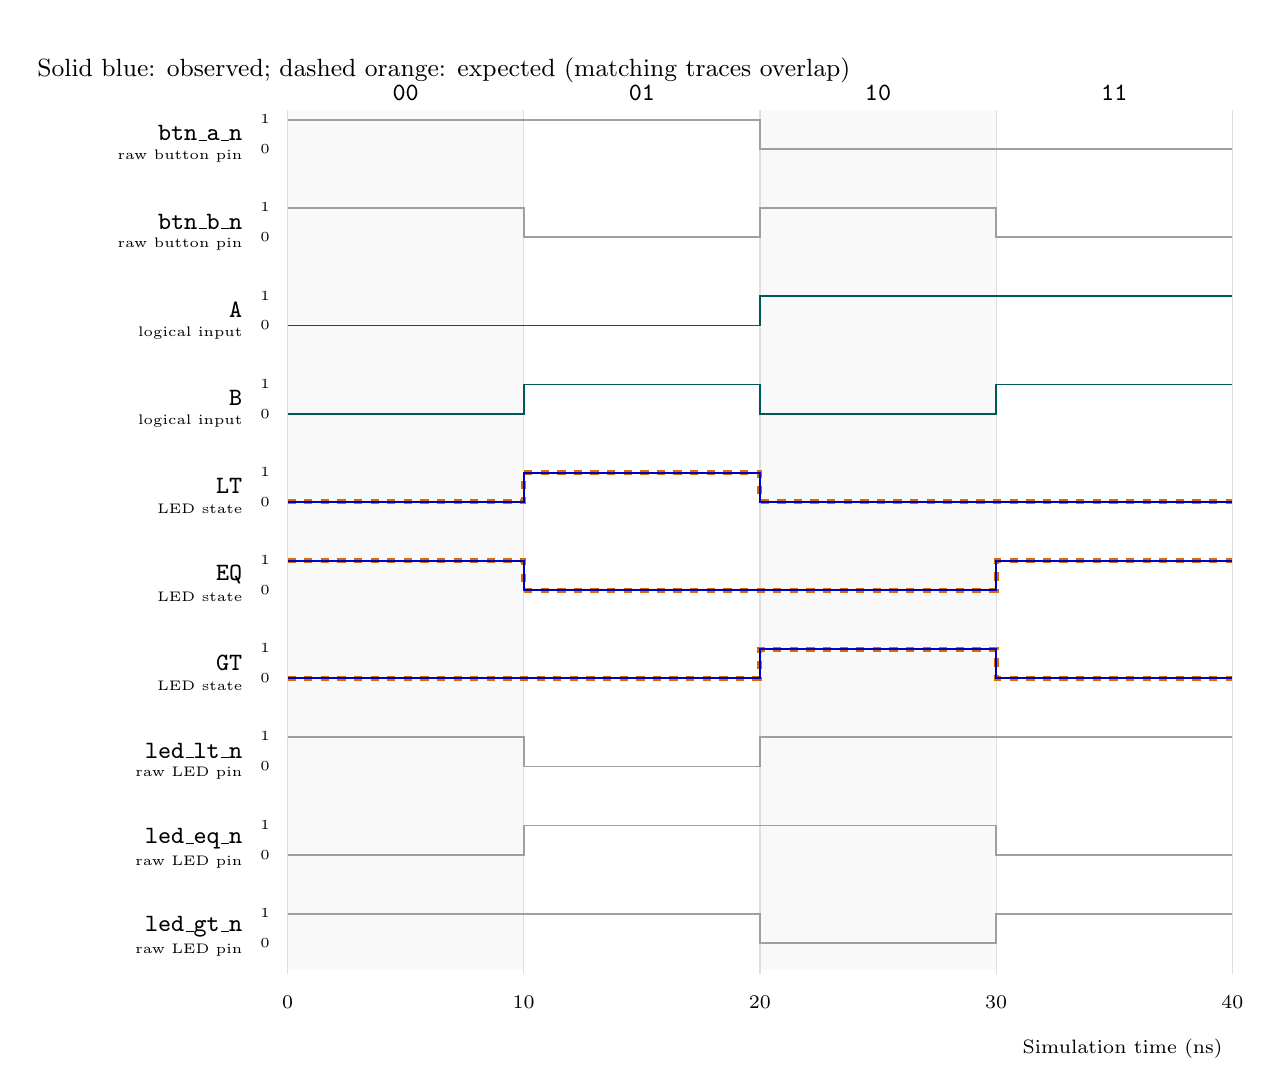
\begin{tikzpicture}[x=1cm,y=1cm,font=\scriptsize]
\path[use as bounding box] (-3.3,-1.1) rectangle (12.3,11.930000000000003);
\node[anchor=west,font=\small] at (-3.3,11.880000000000003) {Solid blue: observed; dashed orange: expected (matching traces overlap)};
\fill[gray!5] (0.0,.45) rectangle (3.0,11.380000000000003);
\node[font=\small\ttfamily] at (1.5,11.600000000000003) {00};
\node[font=\small\ttfamily] at (4.5,11.600000000000003) {01};
\fill[gray!5] (6.0,.45) rectangle (9.0,11.380000000000003);
\node[font=\small\ttfamily] at (7.5,11.600000000000003) {10};
\node[font=\small\ttfamily] at (10.5,11.600000000000003) {11};
\draw[gray!25] (0.0,.4) -- (0.0,11.380000000000003);
\node[below] at (0.0,.25) {0};
\draw[gray!25] (3.0,.4) -- (3.0,11.380000000000003);
\node[below] at (3.0,.25) {10};
\draw[gray!25] (6.0,.4) -- (6.0,11.380000000000003);
\node[below] at (6.0,.25) {20};
\draw[gray!25] (9.0,.4) -- (9.0,11.380000000000003);
\node[below] at (9.0,.25) {30};
\draw[gray!25] (12.0,.4) -- (12.0,11.380000000000003);
\node[below] at (12.0,.25) {40};
\node[anchor=east,font=\small\ttfamily] at (-.45,11.080000000000002) {btn\_a\_n};
\node[anchor=east,font=\tiny] at (-.45,10.790000000000003) {raw button pin};
\node[anchor=east,font=\tiny] at (-.1,11.260000000000003) {1};
\node[anchor=east,font=\tiny] at (-.1,10.880000000000003) {0};
\draw[gray!75,line width=.65pt] (0.0000,11.2500) -- (0.0000,11.2500) -- (0.0000,11.2500) -- (3.0000,11.2500) -- (3.0000,11.2500) -- (3.0000,11.2500) -- (6.0000,11.2500) -- (6.0000,11.2500) -- (6.0000,10.8800) -- (9.0000,10.8800) -- (9.0000,10.8800) -- (9.0000,10.8800) -- (12.0000,10.8800);
\node[anchor=east,font=\small\ttfamily] at (-.45,9.96) {btn\_b\_n};
\node[anchor=east,font=\tiny] at (-.45,9.670000000000002) {raw button pin};
\node[anchor=east,font=\tiny] at (-.1,10.140000000000002) {1};
\node[anchor=east,font=\tiny] at (-.1,9.760000000000002) {0};
\draw[gray!75,line width=.65pt] (0.0000,10.1300) -- (0.0000,10.1300) -- (0.0000,10.1300) -- (3.0000,10.1300) -- (3.0000,10.1300) -- (3.0000,9.7600) -- (6.0000,9.7600) -- (6.0000,9.7600) -- (6.0000,10.1300) -- (9.0000,10.1300) -- (9.0000,10.1300) -- (9.0000,9.7600) -- (12.0000,9.7600);
\node[anchor=east,font=\small\ttfamily] at (-.45,8.840000000000002) {A};
\node[anchor=east,font=\tiny] at (-.45,8.550000000000002) {logical input};
\node[anchor=east,font=\tiny] at (-.1,9.020000000000003) {1};
\node[anchor=east,font=\tiny] at (-.1,8.640000000000002) {0};
\draw[teal!70!black,line width=.65pt] (0.0000,8.6400) -- (0.0000,8.6400) -- (0.0000,8.6400) -- (3.0000,8.6400) -- (3.0000,8.6400) -- (3.0000,8.6400) -- (6.0000,8.6400) -- (6.0000,8.6400) -- (6.0000,9.0100) -- (9.0000,9.0100) -- (9.0000,9.0100) -- (9.0000,9.0100) -- (12.0000,9.0100);
\node[anchor=east,font=\small\ttfamily] at (-.45,7.720000000000002) {B};
\node[anchor=east,font=\tiny] at (-.45,7.430000000000002) {logical input};
\node[anchor=east,font=\tiny] at (-.1,7.900000000000002) {1};
\node[anchor=east,font=\tiny] at (-.1,7.520000000000002) {0};
\draw[teal!70!black,line width=.65pt] (0.0000,7.5200) -- (0.0000,7.5200) -- (0.0000,7.5200) -- (3.0000,7.5200) -- (3.0000,7.5200) -- (3.0000,7.8900) -- (6.0000,7.8900) -- (6.0000,7.8900) -- (6.0000,7.5200) -- (9.0000,7.5200) -- (9.0000,7.5200) -- (9.0000,7.8900) -- (12.0000,7.8900);
\node[anchor=east,font=\small\ttfamily] at (-.45,6.600000000000002) {LT};
\node[anchor=east,font=\tiny] at (-.45,6.310000000000002) {LED state};
\node[anchor=east,font=\tiny] at (-.1,6.780000000000002) {1};
\node[anchor=east,font=\tiny] at (-.1,6.400000000000002) {0};
\draw[orange!85!black,line width=1.8pt,dashed] (0.0000,6.4000) -- (0.0000,6.4000) -- (0.0000,6.4000) -- (3.0000,6.4000) -- (3.0000,6.4000) -- (3.0000,6.7700) -- (6.0000,6.7700) -- (6.0000,6.7700) -- (6.0000,6.4000) -- (9.0000,6.4000) -- (9.0000,6.4000) -- (9.0000,6.4000) -- (12.0000,6.4000);
\draw[blue!75!black,line width=.65pt] (0.0000,6.4000) -- (0.0000,6.4000) -- (0.0000,6.4000) -- (3.0000,6.4000) -- (3.0000,6.4000) -- (3.0000,6.7700) -- (6.0000,6.7700) -- (6.0000,6.7700) -- (6.0000,6.4000) -- (9.0000,6.4000) -- (9.0000,6.4000) -- (9.0000,6.4000) -- (12.0000,6.4000);
\node[anchor=east,font=\small\ttfamily] at (-.45,5.480000000000002) {EQ};
\node[anchor=east,font=\tiny] at (-.45,5.190000000000002) {LED state};
\node[anchor=east,font=\tiny] at (-.1,5.660000000000002) {1};
\node[anchor=east,font=\tiny] at (-.1,5.280000000000002) {0};
\draw[orange!85!black,line width=1.8pt,dashed] (0.0000,5.6500) -- (0.0000,5.6500) -- (0.0000,5.6500) -- (3.0000,5.6500) -- (3.0000,5.6500) -- (3.0000,5.2800) -- (6.0000,5.2800) -- (6.0000,5.2800) -- (6.0000,5.2800) -- (9.0000,5.2800) -- (9.0000,5.2800) -- (9.0000,5.6500) -- (12.0000,5.6500);
\draw[blue!75!black,line width=.65pt] (0.0000,5.6500) -- (0.0000,5.6500) -- (0.0000,5.6500) -- (3.0000,5.6500) -- (3.0000,5.6500) -- (3.0000,5.2800) -- (6.0000,5.2800) -- (6.0000,5.2800) -- (6.0000,5.2800) -- (9.0000,5.2800) -- (9.0000,5.2800) -- (9.0000,5.6500) -- (12.0000,5.6500);
\node[anchor=east,font=\small\ttfamily] at (-.45,4.360000000000002) {GT};
\node[anchor=east,font=\tiny] at (-.45,4.070000000000002) {LED state};
\node[anchor=east,font=\tiny] at (-.1,4.540000000000002) {1};
\node[anchor=east,font=\tiny] at (-.1,4.160000000000002) {0};
\draw[orange!85!black,line width=1.8pt,dashed] (0.0000,4.1600) -- (0.0000,4.1600) -- (0.0000,4.1600) -- (3.0000,4.1600) -- (3.0000,4.1600) -- (3.0000,4.1600) -- (6.0000,4.1600) -- (6.0000,4.1600) -- (6.0000,4.5300) -- (9.0000,4.5300) -- (9.0000,4.5300) -- (9.0000,4.1600) -- (12.0000,4.1600);
\draw[blue!75!black,line width=.65pt] (0.0000,4.1600) -- (0.0000,4.1600) -- (0.0000,4.1600) -- (3.0000,4.1600) -- (3.0000,4.1600) -- (3.0000,4.1600) -- (6.0000,4.1600) -- (6.0000,4.1600) -- (6.0000,4.5300) -- (9.0000,4.5300) -- (9.0000,4.5300) -- (9.0000,4.1600) -- (12.0000,4.1600);
\node[anchor=east,font=\small\ttfamily] at (-.45,3.240000000000002) {led\_lt\_n};
\node[anchor=east,font=\tiny] at (-.45,2.950000000000002) {raw LED pin};
\node[anchor=east,font=\tiny] at (-.1,3.4200000000000017) {1};
\node[anchor=east,font=\tiny] at (-.1,3.040000000000002) {0};
\draw[gray!75,line width=.65pt] (0.0000,3.4100) -- (0.0000,3.4100) -- (0.0000,3.4100) -- (3.0000,3.4100) -- (3.0000,3.4100) -- (3.0000,3.0400) -- (6.0000,3.0400) -- (6.0000,3.0400) -- (6.0000,3.4100) -- (9.0000,3.4100) -- (9.0000,3.4100) -- (9.0000,3.4100) -- (12.0000,3.4100);
\node[anchor=east,font=\small\ttfamily] at (-.45,2.120000000000002) {led\_eq\_n};
\node[anchor=east,font=\tiny] at (-.45,1.8300000000000016) {raw LED pin};
\node[anchor=east,font=\tiny] at (-.1,2.3000000000000016) {1};
\node[anchor=east,font=\tiny] at (-.1,1.9200000000000017) {0};
\draw[gray!75,line width=.65pt] (0.0000,1.9200) -- (0.0000,1.9200) -- (0.0000,1.9200) -- (3.0000,1.9200) -- (3.0000,1.9200) -- (3.0000,2.2900) -- (6.0000,2.2900) -- (6.0000,2.2900) -- (6.0000,2.2900) -- (9.0000,2.2900) -- (9.0000,2.2900) -- (9.0000,1.9200) -- (12.0000,1.9200);
\node[anchor=east,font=\small\ttfamily] at (-.45,1.0000000000000007) {led\_gt\_n};
\node[anchor=east,font=\tiny] at (-.45,0.7100000000000007) {raw LED pin};
\node[anchor=east,font=\tiny] at (-.1,1.1800000000000006) {1};
\node[anchor=east,font=\tiny] at (-.1,0.8000000000000007) {0};
\draw[gray!75,line width=.65pt] (0.0000,1.1700) -- (0.0000,1.1700) -- (0.0000,1.1700) -- (3.0000,1.1700) -- (3.0000,1.1700) -- (3.0000,1.1700) -- (6.0000,1.1700) -- (6.0000,1.1700) -- (6.0000,0.8000) -- (9.0000,0.8000) -- (9.0000,0.8000) -- (9.0000,1.1700) -- (12.0000,1.1700);
\node[anchor=east] at (12,-.55) {Simulation time (ns)};
\end{tikzpicture}\end{center}
{\small All initial truth-table intervals agree. Logical signals: 1 = pressed/on; raw pins: 0 = pressed/on. The complete saved VCD contains 36 stable observations and zero disagreements. The plot shows settled interval values and does not resolve delta-cycle glitches.}\par

{\small\raggedright Figure 1-2.4. Actual VCD outputs and mathematical expectations; overlapping traces agree. Raw active-low pins are also shown.\par}

{\small\raggedright Logical signals use pressed/on = 1. Raw pins use pressed/on = 0. This comparison supports Table 1-2.5 and the active-low explanation in Table 1-2.2.\par}

\clearpage

\section*{Lab 1-2 | Board test and conclusion}

{\small\raggedright The mapped RTL was built with Verilator and displayed in the local SDL2 board window. The local input-support modification allows simultaneous states: keys 2 and 3 toggle B2 and B3; key 4 also toggles B4 for the adder; key 0 releases all inputs. This simulator adjustment does not change the task RTL [7].\par}

{\small\raggedright Table 1-2.6 records every visible case checked in the live window.\par}

\begingroup\small\setlength{\tabcolsep}{4pt}
\renewcommand{\arraystretch}{1.20}
\noindent\begin{tabular}{@{}p{\dimexpr0.205882\linewidth-3.2941pt\relax}p{\dimexpr0.558824\linewidth-8.9412pt\relax}p{\dimexpr0.235294\linewidth-3.7647pt\relax}@{}}
\toprule
\textbf{Logical inputs} & \textbf{Expected visible result} & \textbf{Observed} \\
\midrule
00 & LED2 only & PASS \\
01 & LED1 only & PASS \\
10 & LED3 only & PASS \\
11 & LED2 only & PASS \\
\bottomrule
\end{tabular}\par\endgroup
\vspace{2mm}

{\small\raggedright Table 1-2.6. Itemized virtual-board observations.\par}

{\small\raggedright Required public board-video link: \url{https://github.com/zhihanyu123/EIE330-Lab1-FullAdder-Comparator/blob/main/EIE330_Lab1_2_Comparator_Short.webm}.\par}

{\small\raggedright Local recording in the project bundle: full\_adder/evidence/virtual\_board-screen0.webm\par}

{\small\raggedright The comparator recording retains its original capture path under full\_adder/evidence; its recorded content is the comparator demonstration.\par}

{\small\raggedright Other board signals do not connect to the task module. The wrapper sets unused LEDs off and unused VGA outputs to inactive defaults.\par}

\subsection*{Discussion and conclusion}

{\small\raggedright The final one-bit digital comparator met all 4 required simulation and virtual-board cases. Yosys found no stored state. Simulation checks ideal Boolean behavior; generic synthesis does not establish fitted FPGA resources. These results validate the logic in software simulation and the virtual board. Physical FPGA operation and propagation delay were not measured.\par}

\subsection*{References}

{\small\raggedright [1] Macau University of Science and Technology, "EIE330 FPGA-based System Design - Lab 1 Requirements," course handout, accessed Oct. 8, 2026.\par}

{\small\raggedright [2] Macau University of Science and Technology, "EIE330 FPGA-based System Design: Lab 1-1 Simple LED Circuit," lecture slides, updated Oct. 5, 2026, accessed Oct. 8, 2026.\par}

{\small\raggedright [3] Altera Corporation, "Cyclone IV FPGA Device Family Overview," Cyclone IV Device Handbook, vol. 1, doc. CYIV-51001-2.0, Mar. 2016, Tables 1-1, 1-3 and Fig. 1-3.\par}

{\small\raggedright [4] Dongguan EmbedFire Electronic Technology Co., Ltd., "Wildfire EP4CE10 Pro schematic diagram," rev. V1.0, Sep. 14, 2023.\par}

{\small\raggedright [5] Icarus Verilog contributors, "Getting Started With Icarus Verilog." [Online]. Available: \url{https://steveicarus.github.io/iverilog/usage/getting_started.html}. Accessed: Oct. 8, 2026.\par}

{\small\raggedright [6] YosysHQ, "Synthesis starter." [Online]. Available: \url{https://yosyshq.readthedocs.io/projects/yosys/en/latest/getting_started/example_synth.html}. Accessed: Oct. 8, 2026.\par}

{\small\raggedright [7] pikipity, "Simple-VGA-Simulator," GitHub repository. [Online]. Available: \url{https://github.com/pikipity/Simple-VGA-Simulator}. Accessed: Oct. 8, 2026. Local input support is based on the saved source archive.\par}

{\small\raggedright [8] Massachusetts Institute of Technology, "Lectures 8/9," 6.111 Introductory Digital Systems Laboratory, Spring 2006, slides 5, 8. [Online]. Available: \url{https://web.mit.edu/6.111/www/s2006/LECTURES/l8_9.pdf}. Accessed: Oct. 8, 2026.\par}

\end{document}
